\documentclass[a4paper,11pt]{article}

\parindent0cm
\usepackage
[backend=biber,style=apa,sorting=nyt]
{biblatex}
\addbibresource{literature.bib}

\makeatletter
\newcommand\notsotiny{\@setfontsize\notsotiny{8}{8}}
\newcommand\micro{\@setfontsize\notsotiny{4.5}{4.5}}
\newcommand\middletiny{\@setfontsize\notsotiny{6}{6}}
\makeatother

%\renewcommand{\symheadingname}{Symbolverzeichnis}

%\usepackage[colorlinks=true,
%breaklinks = true,
%citecolor=black,
%linkcolor=blue,
%menucolor=black,
%urlcolor=blue]{hyperrref}
\usepackage[]{acronym}


\usepackage[draft]{listofsymbols}
\usepackage[utf8]{inputenc}
\usepackage{csquotes}
\usepackage{array}
\usepackage{dirtytalk}
\usepackage{amsmath}
\usepackage{multirow}
%\usepackage[table]{xcolor}
\usepackage{bm}
\usepackage{amssymb}
\usepackage{amsthm}
\usepackage{amsfonts}
\usepackage{color}
\usepackage{layouts}
% printing the textsize used
% \printinunitsof{cm}
% \prntlen{\textwidth}
\usepackage[usenames,dvipsnames]{xcolor}
\usepackage{tabularx}
\usepackage{graphicx}
\usepackage{pdfpages}
\usepackage[ngerman]{babel}
\usepackage[left=3cm,right=2.5cm,top=2cm,bottom=2cm]{geometry}
\renewcommand{\baselinestretch}{1.5}\normalsize % Zeilenabstand 1.5

%% symbolverzeichnis
%\opensymdef
%\newsym[Elementweises Produkt]{}{\circ}
%\closesymdef
%%

\begin{document}

\begin{titlepage}

\vspace*{3cm}


\begin{figure}[t]
\begin{flushright}
\includegraphics[width = 7cm,  keepaspectratio]{Images/TULogo.png}


\end{flushright}
\end{figure}
\vspace*{3cm}


\begin{center}

\vspace*{2cm}

\title{Masterthesis}



{\huge Masterthesis}\\
 {\huge{\textbf{\textit{Multiclass}-Klassifizierung \\
 von Nachrichten Schlagzeilen}}\\}
 \vspace{0.2cm}
 {\large  Vergleich zwischen neuronalen Netzen und baumbasierten Algorithmen auf verschiedenen Repräsentationen von Wörtern\\}
\vspace*{5cm}


{\large  Fakultät Statistik\\
Lehrstuhl Statistical Methods for Big Data }
\vspace*{0.5cm}

 \begin{large}
 Betreuer: Prof. Dr. Andreas Groll\\
  \end{large}

  \begin{large}
Verfasser: Marc Schmieder\\
\date{October 2019}
   \vspace*{2cm}

 \end{large}
\end{center}
\newpage
%\large
\thispagestyle{empty}
\tableofcontents
\newpage

\addsec{\large{Abkürzungsverzeichnis}}
\label{sec:abkuerz}

\begin{acronym}[TF-IDF]
\acro{lstm}{longshort}
\acro{TF-IDF}{longshort}
\end{acronym}

\newpage

\end{titlepage}







\section{Einleitung}



\section{Datensatz und Problemstellung}

In diesem Kapitel wird der für diese Thesis relevante Datensatz vorgestellt. Nach dessen Bereinigung erfolgt eine Exploration und anschließend die Darlegung der Zielstellung dieser Thesis.


\subsection{Initialer Datensatz}

Der Datensatz trägt den Titel \textit{News Category Dataset} (\cite{dataset}) und stammt von der Machine Learning Plattform \textit{Kaggle}. Er umfasst $200853$ Beobachtungen, die Informationen in englischer Sprache über Artikel der US-Amerikanischen Onlinezeitung \textit{Huffpost} enthalten. Der Zeitraum, in dem die Veröffentlichungen stattgefunden haben, erstreckt sich vom 28.01.2012 bis zum 25.05.2018, also über eine Zeitspanne von über $6$ Jahren. Die Inhalte der Artikel sind lediglich verlinkt und nicht direkt im Datensatz enthalten. Für jeden Artikel ist die Nachrichtenschlagzeile des Artikels angegeben. Zusätzlich zu dem Link des Artikels ist für jeden Datenpunkt das Veröffentlichungsdatum, der Name des Autors, eine Kurzbeschreibung und die Nachrichtenkategorie gegeben. Letzteres ist die Zielvariable (genauere Erläuterung in Kapitel \ref{Kap:Zielst}), die $41$ verschiedene Ausprägungen annimmt. Die Kurzbeschreibung enthält ähnliche Informationen wie die Nachrichtenüberschrift und ist nur teilweise vorhanden. Für die Beantwortung der Fragestellung (Kapitel \ref{Kap:Zielst}) soll nur die Schlagzeile als abhängige Variable in die Modellierung eingehen. Bevor eine Exploration des Datensatz erfolgt, werden im nächsten Abschnitt vorgenommene Änderungen an den relevanten Variablen Nachrichtenkategorie und Nachrichtenschlagzeile aufgelistet und begründet.


\subsection{Änderungen am Datensatz} \label{kap:2_2Aend}

In der englischen Sprache spielt die Groß- und Kleinschreibung außer bei der Nutzung von Personalpronomen keine Rolle. Deshalb werden in den Texten alle Großbuchstaben zu Kleinbuchstaben konvertiert. Auf diese Weise werden in der Modellierung beispielsweise die Wörter \textit{Teacher} und \textit{teacher} nicht unterschiedlich behandelt. \\
\\
Die Artikel wurden vermutlich von einigen Autoren in unterschiedlichen Ländern geschrieben, denn die Texte enthalten unterschiedliche Zeichensätze. Bei der verwendeten \texttt{utf8} Enkodierung entstanden bei unbekannten Zeichen Konvertierungsfehler (z.b. der Form \say{a@S}). Diese wurden durch Leerzeichen ersetzt. In dem Wissen, dass die Wörter des Textkorpus mit den \textit{Global Word Vectors} (Kapitel \ref{Kap:Glove}) abgeglichen werden, wurden einige Begriffe so ersetzt, dass bestimmte Wörter in den \textit{Global Word Vectors} gefunden werden. Zuerst erfolgte eine Entfernung von Sonderzeichen wie beispielsweise \say{©} oder \say{™}. Dann folgte die Ersetzung von Verneinungen wie zum Beispiel \say{n't} durch \say{ not}. Analog wurden \say{'ll} durch \say{ will} und \say{'ve} durch \say{ have} ersetzt. Kurzformen der Form \say{here's} wurden zu \say{here is} geändert, da sonst die Wörter mit Endung \say{'s} so als eigenständige Wörter repräsentiert werden und nicht sinngemäß als Tupel. Häufig vorkommende Eigennamen mit analoger Endung \say{trump's} wurden durch \say{trump his} ausgetauscht. Nachdem Vorkommnisse der Art \say{here's} entfernt wurden, können nun Vorkommnisse der Art \say{john's son} durch \say{john its son} ersetzt werden. So ist bei Wörtertupeln dieser Art zwar nicht das Geschlecht von John bekannt, aber zumindest offensichtlich, dass der Sohn John zugehörig ist. Nach der Bereinigung des Textkorpus wurden letztendlich noch $6$ Schlagzeilen entfernt, die keine Wörter mehr enthalten. Es verbleiben nun also insgesamt $200847$ Beobachtungen.\\
\\
Nach der umfangreichen Bereinigung des Schlagzeilen-Textkorpus liegt nun die Zielvariable Nachrichtenkategorie im Fokus.
Bei genauerer Betrachtung der $41$ Kategorien fällt auf, dass diese teilweise bereits namentlich sehr ähnlich ausfallen. In Tabelle \ref{tab:parentsMerge} sind beispielhaft $4$ Schlagzeilen der Kategorien \textit{parents} und \textit{parenting} aufgeführt.

\begin{table}[ht]
\begin{center}
\begin{tabular}{ | p{0.1 \textwidth} | p{0.42 \textwidth}| p{0.42 \textwidth} | }
  \hline
Beispiel & Kategorie \textit{parents}  & Kategorie \textit{parenting} \\ 
  \hline
1 & 40 tweets that sum up life with 4-year-olds & a baby book of disasters \\ 
  2 & these were the trendiest baby names in the late '80s & it is time to find your tribe \\ 
  3 & these quotes from kids are hilarious, adorable and oddly insightful & help huffpost parents win a webby award! \\ 
  4 & 30  'star wars'-inspired names parents are giving their babies & why our 'imperfect' moments are perfect to our children \\ 
   \hline
\end{tabular}
\caption{Beispiele für Schlagzeilen der Kategorien \textit{parents} und \textit{parenting}}
\label{tab:parentsMerge}
\end{center}
\end{table}

Anhand der Beispiele wird deutlich, dass es schwierig ist, diese mit menschlicher Intuition eine der beiden Kategorien eindeutig zuzuordnen. Als zusätzlicher Indikator, der für die Verschmelzung zweier Kategorien spricht, erfolgte die Betrachtung der relativen Schnittmenge der gemeinsamen häufigsten Wörter. Die häufigsten Wörter pro Kategorie wurden ermittelt, indem die kompletten Daten auf die entsprechende Kategorie gefiltert werden, anschließend Symbole und \textit{stopwords} (Wörter wie \say{he}, \say{is} oder \say{through}, die komplette Liste ist im Anhang unter (todo:referenzieren) zu finden) entfernt und die Wörter nach der gesamten Anzahl ihres Auftretens sortiert werden. Tabelle \ref{tab:categoryMerge} zeigt die relative Schnittmenge der $100$ häufigsten Wörter für ausgewählte Paare an Kategorien.

\begin{table}[ht]
\begin{center}
\begin{tabular}{|l|l|c|c|}
  \hline
Kategorie 1 & Kategorie 2  & relative Schnittmenge & neue Kategorie\\
  \hline
\textit{healthy living} & \textit{wellness} & 0.76 & \textit{wellness \& healthy living} \\ 
  \textit{parents} & \textit{parenting} & 0.74 & \textit{parents} \\ 
  \textit{taste} & \textit{food \& drink} & 0.70 & \textit{food, drink \& taste}\\ 
  \textit{world news} & \textit{the worldpost} & 0.68 & \textit{world news}\\ 
  \textit{arts} & \textit{culture \& arts} & 0.60 & \textit{arts \& culture}\\ 
  \textit{style} & \textit{style \& beauty} & 0.58 & \textit{style \& beauty} \\ 
  \textit{the worldpost} & \textit{worldpost} & 0.58 & \textit{world news}\\ 
  \textit{world news} & \textit{worldpost} & 0.55 & \textit{world news}\\ 
  \textit{green} & \textit{environment} & 0.53 & \textit{green \& environment}\\ 
  \textit{fifty} & \textit{parenting} & 0.50 & -\\ 
    \vdots & \vdots & \vdots & -\\
  \textit{parents} & \textit{fifty} & 0.48 & - \\ 
  \textit{arts \& culture} & \textit{arts} & 0.46 & \textit{arts \& culture}\\  
  \vdots & \vdots & \vdots & -\\
  \textit{world news} & \textit{home \& living} & 0.05 & - \\ 
  \textit{crime} & \textit{food \& drink} & 0.04 & -\\
  \hline 
  \hline 
  \multicolumn{2}{|c|}{Mittelwert} &  0.24 & \\
   \hline
\end{tabular}
\caption{Relative Schittmenge der $100$ häufigsten Wörter für Paare an Kategorien}
\label{tab:categoryMerge}
\end{center}
\end{table}

Die ersten $10$ Zeilen von Tabelle \ref{tab:categoryMerge} beinhalten Kategorien, die eine relative Schnittmenge der gemeinsamen Wörter von $0.50$ oder höher haben. In den letzten beiden Zeilen ist zu sehen, dass inhaltlich verschiedene Kategorien eine vergleichbar geringe Schnittmenge an häufigsten Wörtern haben. Im Mittel hat ein Paar an Kategorien eine gemeinsame Schnittmenge von $0.24$. Dieser Wert wirkt hoch, da \textit{stopwords} und Sonderzeichen bereits entfernt wurden.
Das Grenze, ab der $2$ Kategorien zusammengelegt werden, wird bei einer Überschneidung von $50$ Prozent angesiedelt. Es werden dennoch $2$ Ausnahmen gebildet. \textit{parents} und \textit{fifty} werden nicht zusammengelegt, da \textit{fifty} sowohl von \textit{parents} und \textit{parenting} mit menschlicher Intuition unterscheidbar ist (siehe todo: referenzieren). Als andere Ausnahme wird das Paar \textit{arts \& culture} und \textit{arts} mit einer Überschneidung von $0.46$ zusammengelegt, da bereits \textit{arts} und \textit{culture \& arts} fusioniert wurden.\\
Mit den Argumenten der menschlichen Intuition und der Ergebnisse aus Tabelle \ref{tab:categoryMerge} wurden in folgenden Fällen die Kategorien zusammengelegt:
Die Kategorien \textit{healthy living} und \textit{wellness} wurden zu \textit{wellness \& healthy living}; \textit{parents} und \textit{parenting}  zu \textit{parents}; \textit{taste} und \textit{food \& drink} zu \textit{food, drink \&taste}; \textit{arts}, \textit{culture \& arts} und \textit{arts \& culture} zu \textit{arts \& culture}; \textit{the worldpost}, \textit{worldpost} und \textit{world news} zu \textit{world news}; \textit{style} und \textit{style \& beauty} zu \textit{style \& beauty};  sowie \textit{green} und \textit{environment} zu \textit{green \& environment}. Beispiele analog zu \ref{tab:parentsMerge} für die anderen zusammengelegten Kategorien finden sich im Anhang (todo verlinken, auflisten). Die $41$ Kategorien wurden somit auf $32$ Kategorien reduziert, welche inhaltlich mit menschlicher Intuition unterscheidbar sind. Nach den Modifikationen folgt im nächsten Abschnitt eine Exploration des Datensatzes.

\subsection{Exploration des bereinigten Datensatzes}

Von großem Interesse ist die Verteilung der Nachrichtensparten im kompletten bereinigten Datensatz.
Abbildung \ref{abb:barplotCategories} zeigt die absoluten Anzahlen der Datenpunkte pro Nachrichtenkategorie. 

\begin{figure}[ht]
    \centering
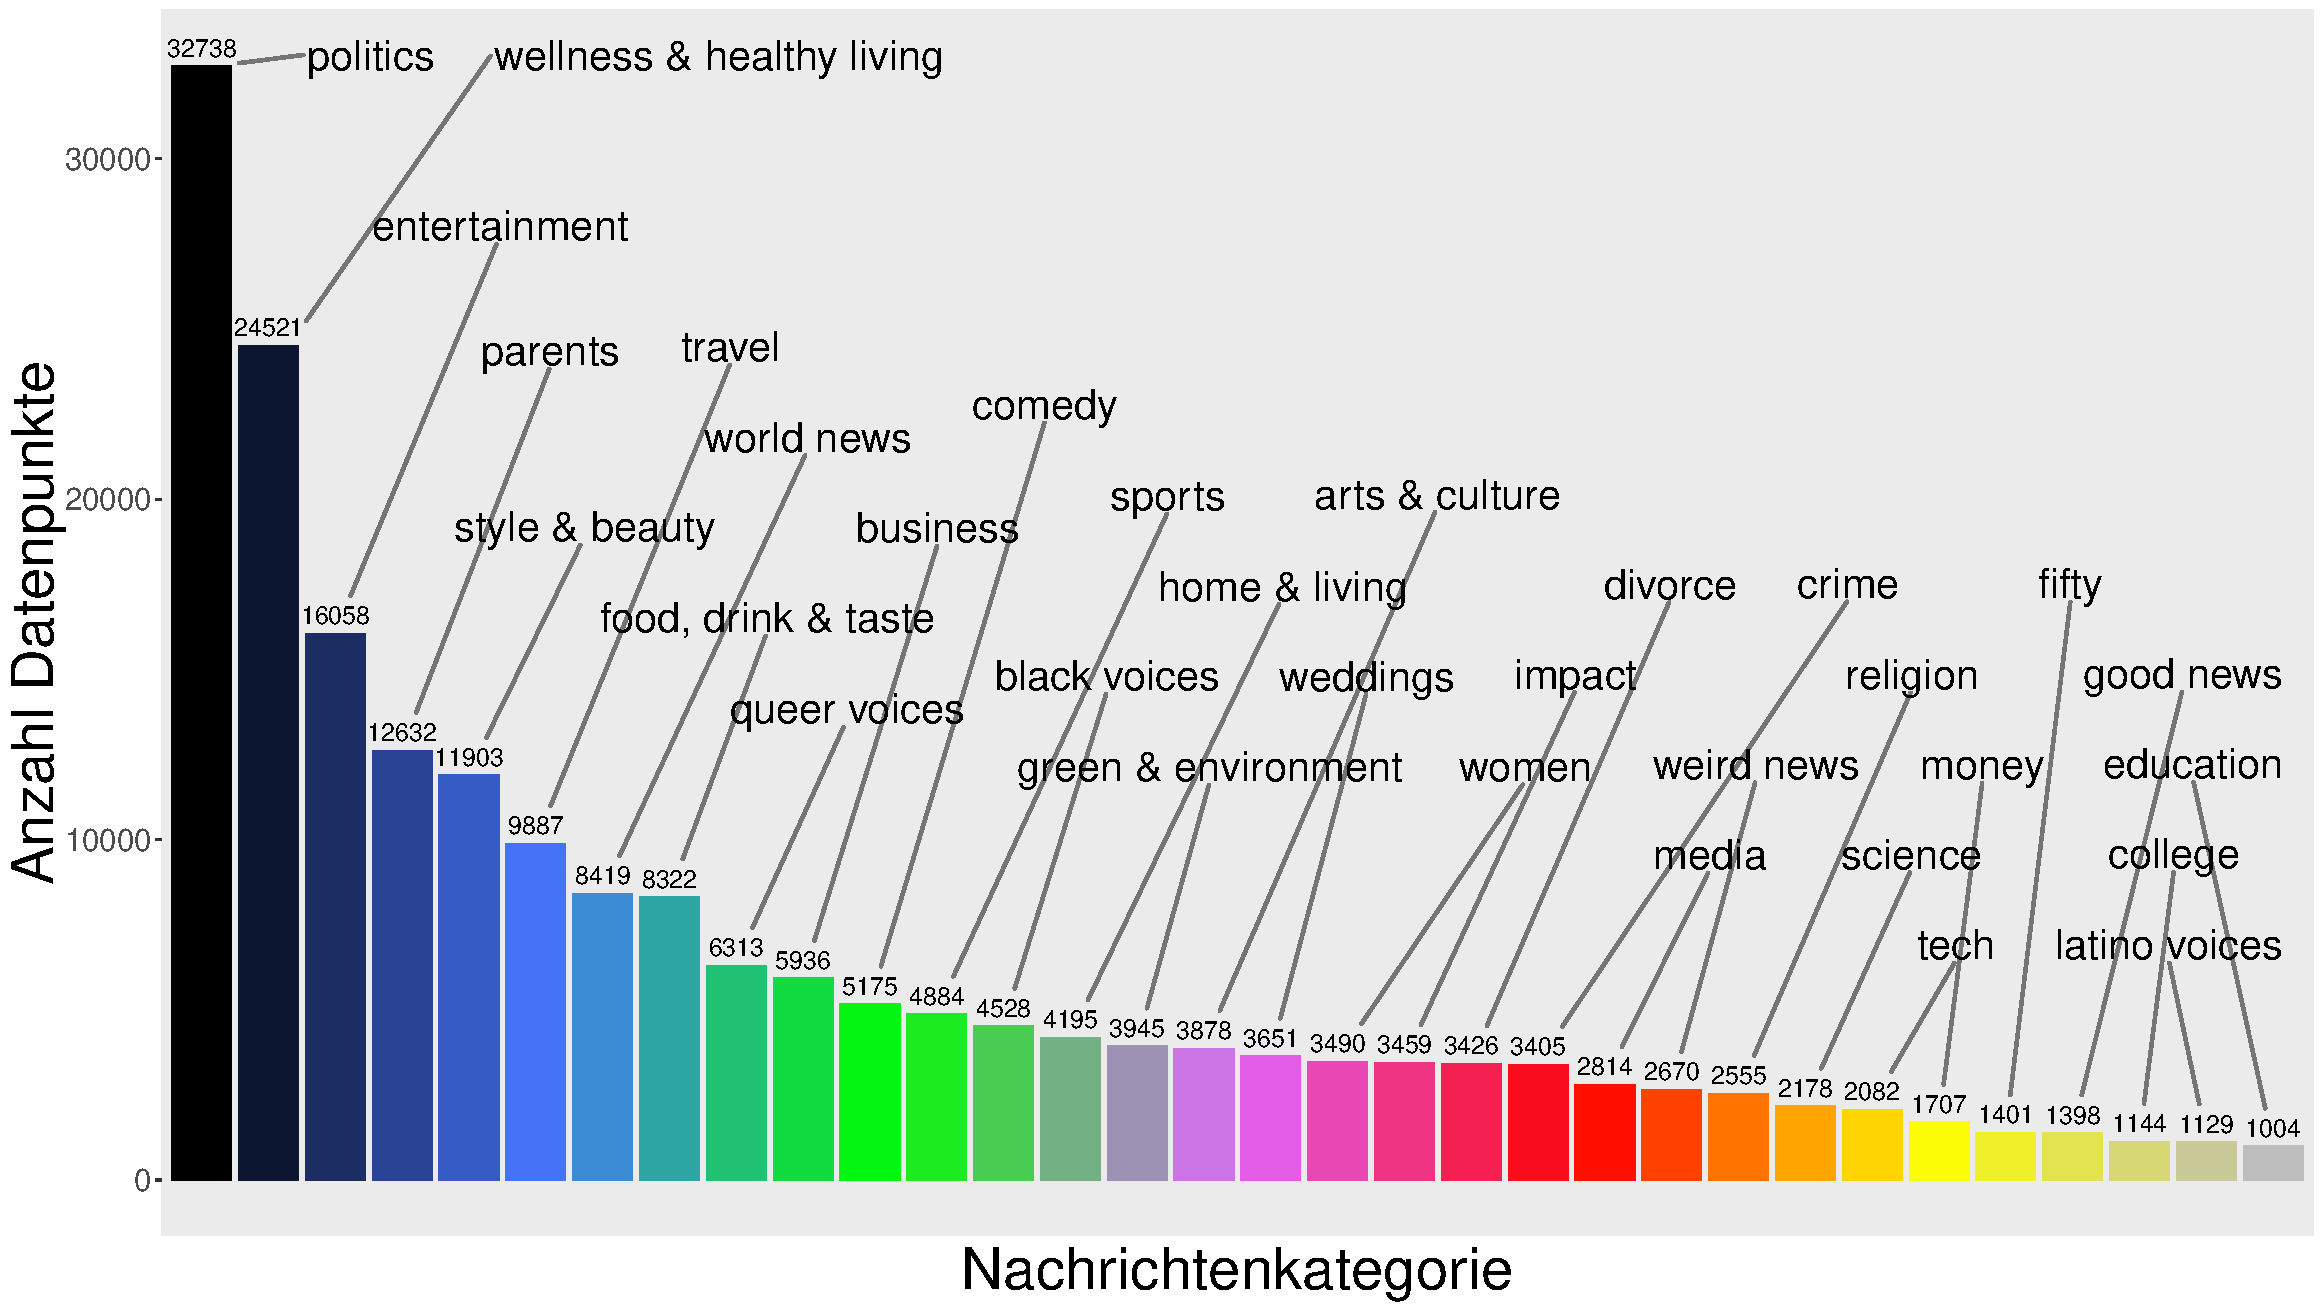
\includegraphics[width = \textwidth,  keepaspectratio]{Images/barplotCategories.pdf} 
\caption{Anzahl Datenpunkte pro Nachrichtenkategorie}
\label{abb:barplotCategories}
\end{figure}

Es ist festzustellen, dass die Kategorien keineswegs ausgeglichen vorliegen. Die häufigste Kategorie stellt \textit{politics} dar mit $32738$ Datenpunkten. Zweit- und dritthäufigste Kategorien sind \textit{wellness \& healthy living} und \textit{entertainment} mit $24521$ und $16058$ Beobachtungen. Die Nachrichtensparten mit den wenigsten Artikeln bilden \textit{college}, \textit{latino voices} und \textit{education} mit $1144$, $1129$ und $1004$ Beobachtungen.\\
Die ersten $6$ Kategorien stellen bereits $53.6$ Prozent der gesamten Beobachtungen dar. Durchschnittlich beinhaltet eine Kategorie $6276.47$ Nachrichtenschlagzeilen.\\
\\
Es folgt nun eine gesamtheitliche Exploration des Textkorpus der Schlagzeilen. Im Rahmen der Analyse zählen Symbole sämtlicher Art auch als Wörter. Die kürzeste Überschrift des Datensatzes enthält nur $1$ Wort, während die längste $82$ Wörter umfasst. Durchschnittlich enthält eine Artikel-Schlagzeile $11.022$ Wörter. Das Vokabular aller Schlagzeilen umfasst $58717$ Wörter, wobei \say{the} das häufigste Wort ist und in $54139$ Artikelüberschriften vorkommt. $24372$ Wörter kommen nur einmal vor. In der Betrachtung der mittleren Wortanzahlen pro Kategorie fällt auf, dass diese differieren. Die Kategorie mit der höchsten durchschnittlichen Anzahl von $12.724$ Wörtern ist \textit{style \& beauty}. Die Kategorie, bei der sich die Autoren durchschnittlich am kürzesten fassen, ist \textit{wellness \& healthy living} mit $9.367$ Wörtern. Eine weitere interessante Fragestellung ist, ob in den Kategorien bestimmte Sonderzeichen oder Symbole besonders häufig oder selten vorkommen. Abbildung \ref{abb:barplotSymbols} zeigt die relative Anzahl der Vorkommnisse verschiedener Symbole in den Schlagzeilen pro Kategorie.

\begin{figure}[ht]
    \centering
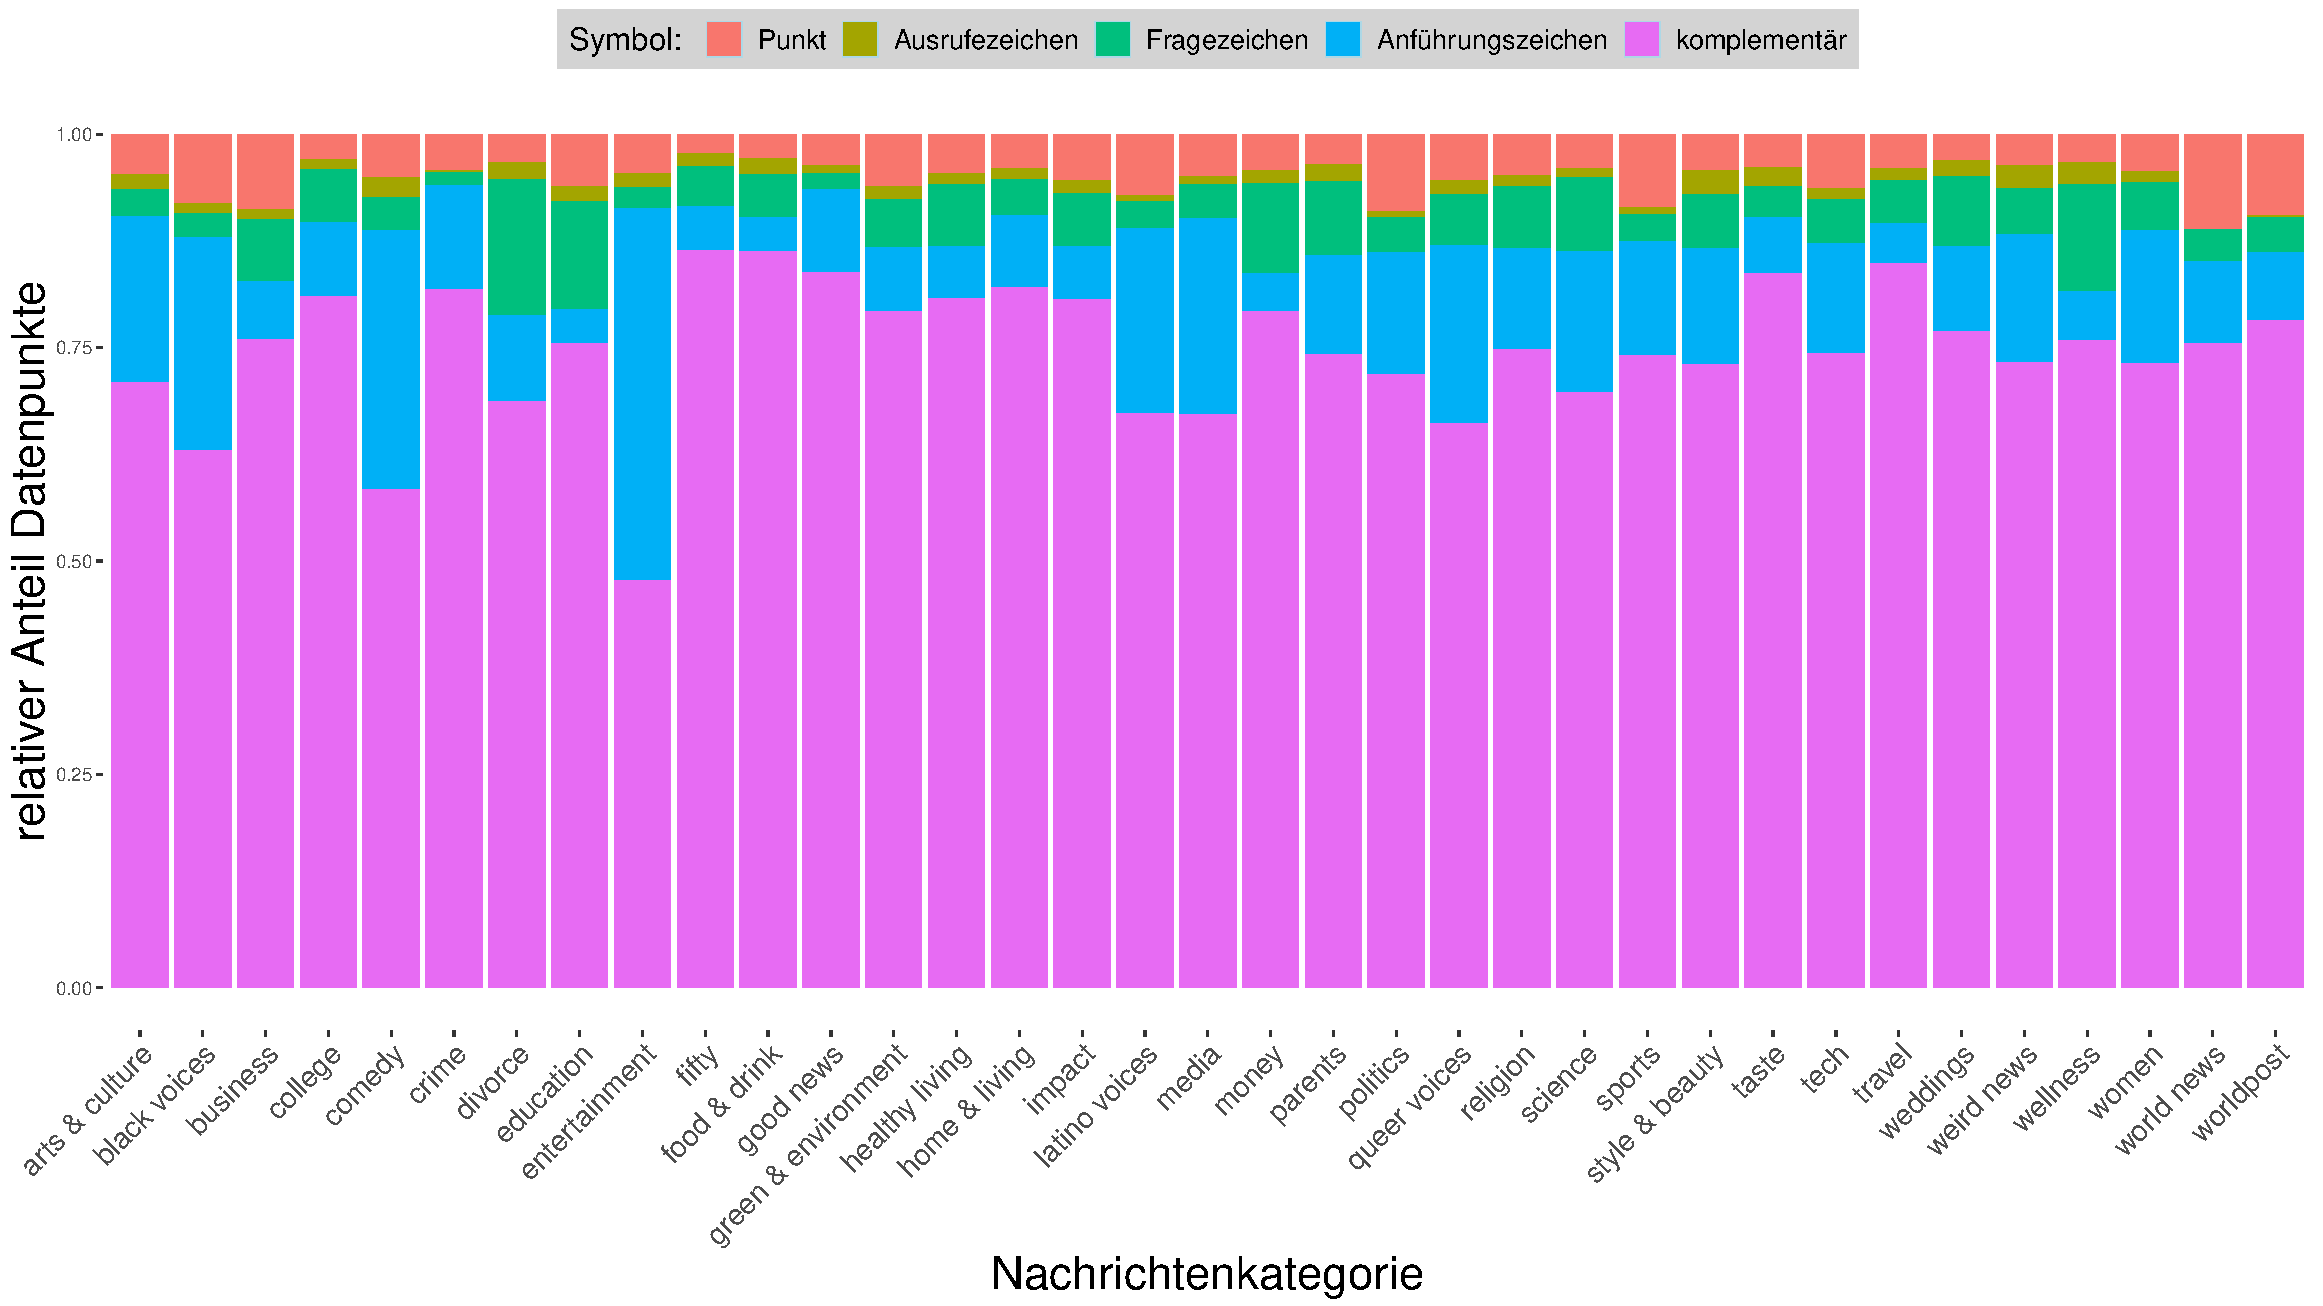
\includegraphics[width = \textwidth,  keepaspectratio]{Images/barplotSymbols.pdf} 
\caption{Relativer Anteil Datenpunkte mit Sonderzeichen pro Kategorie}
\label{abb:barplotSymbols}
\end{figure}

Ein Wert von beispielsweise $0.15$ für eine bestimmte Nachrichtensparte in der Grafik ist so zu interpretieren, dass in $15$ Prozent aller Schlagzeilen dieser Kategorie das entsprechende Symbol mindestens einmal aufgetaucht ist. Die im Folgenden beschriebenen Durchschnitte sind Mittelwerte über die Kategorien und nicht über den gesamten Datensatz. Betrachtet sei nun das Vorkommen eines Punktes in einer Schlagzeile. Dieses kann so interpretiert werden, dass eine Schlagzeile mehrere Sätze enthält. Dies ist insgesamt mit einem durchschnittlichen relativen Anteil von $0.050$ selten der Fall. In der Sparte \textit{world news} kommen mehrere Sätze mit $0.098$ am häufigsten vor, in \textit{fifty} mit $0.021$ am wenigsten. Der Mittelwert für Ausrufezeichen beträgt $0.015$ und die Kategorie \textit{style \& beauty} nimmt das Maximum mit $0.028$, die Kategorie \textit{world news} das Minimum mit $0.002$ an. Fragezeichen kommen in durchschnittlich $0.059$ der Schlagzeilen vor, dabei am häufigsten in \textit{divorce} mit $0.159$ und am seltensten mit $0.015$ in \textit{crime}. Anführungszeichen sind mit durchschnittlich $0.133$ von den hier betrachteten Satzzeichen am meisten vertreten. Sie wurden besonders oft mit $0.437$ in der \textit{entertainment} Sparte genutzt und kamen am seltensten mit $0.040$ in \textit{education} zum Einsatz. Die Rubrik \say{komplementär} gibt an, zu welchem relativen Anteil keine der betrachteten Symbole vorkommt. Durchschnittlich enthalten $0.743$ der Kategorien keine der hier betrachteten Sonderzeichen. Hier ist zu sehen, dass Kategorien wie \textit{entertainment}, \textit{comedy}, \textit{black voices} oder \textit{divorce} häufig Symbole beinhalten, die einen dramatischen Charakter ausdrücken. Sparten wie \textit{fifty}, \textit{food, drink \& taste} und \textit{travel} bleiben mit wenig Symbolen sachlicher. Abbildung \ref{abb:barplotSymbols} zeigt insgesamt, dass Symbole für die Kategorisierung der Nachrichtensparten wichtig sind und im Rahmen der in Kapitel \ref{Kap:Tfidf} beschriebenen \textit{bag-of-words} und \textit{tf-idf}  Methoden nicht entfernt werden sollten.

\begin{figure}[ht]
    \centering
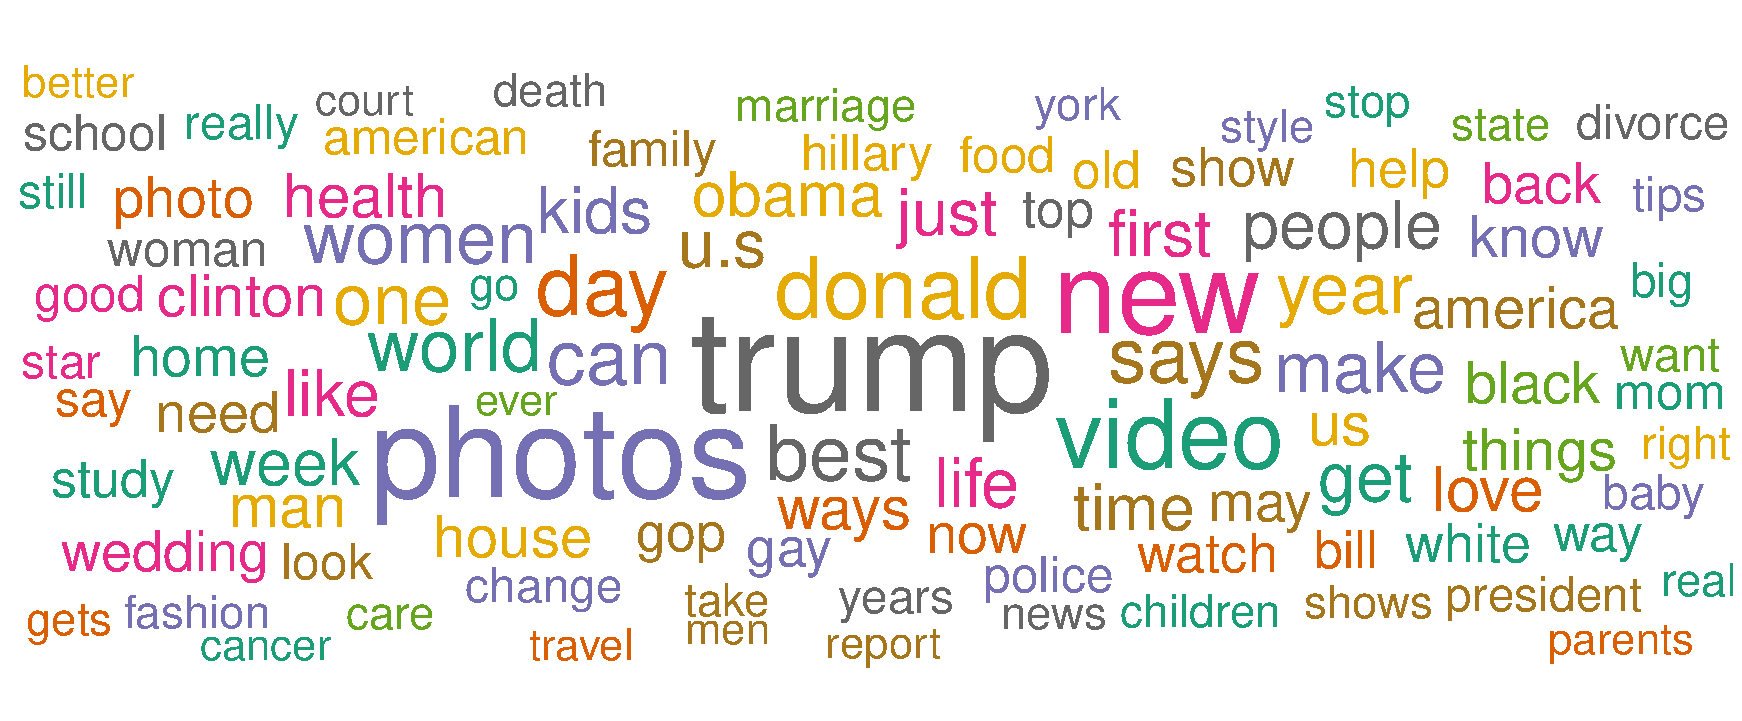
\includegraphics[width = \textwidth,  keepaspectratio]{Images/wordCloudAll.pdf} 
\caption{\textit{wordcloud} für die häufigsten 100 Wörter aller Kategorien}
\label{abb:WordcloudAll}
\end{figure}
todo: grafik gescheit ausfüllen

Je größer ein Wort, desto häufiger kommt es insgesamt im Textkorpus vor. Es ist erstaunlich, dass \say{trump} sich über den gesamten Textkorpus als häufigstes Wort etabliert hat, in Anbetracht dessen, dass sich der Zeitraum der Daten auf über $6$ Jahre erstreckt. Die $3$ häufigsten Wörter danach sind \say{photos}, \say{new} und \say{video}. Das überraschend sehr häufige Vorkommen der Wörter \say{photos} und \say{video} könnte ein Indiz dafür sein, dass in einigen Schlagzeilen bereits die Quelle des Medienmaterials angegeben ist, das im Artikel erscheint. Es ist zu sehen, dass viele Namen und Begriffe aus der Politik zu sehen sind, was einleuchtend ist, da \textit{politics} die größte Sparte darstellt. 
Auffallend ist außerdem, dass viele der auftauchenden Begriffe identisch oder fast identisch zu den Namen einiger Kategorien sind. Beispiele dafür sind \say{travel}, \say{wedding}, \say{style} oder \say{parents}. In Abbildung \ref{abb:WordcloudWellness} ist eine weitere \textit{Wordcloud} der zweitgrößten Sparte \textit{wellness \& healthy living} zu sehen.

\begin{figure}[ht]
    \centering
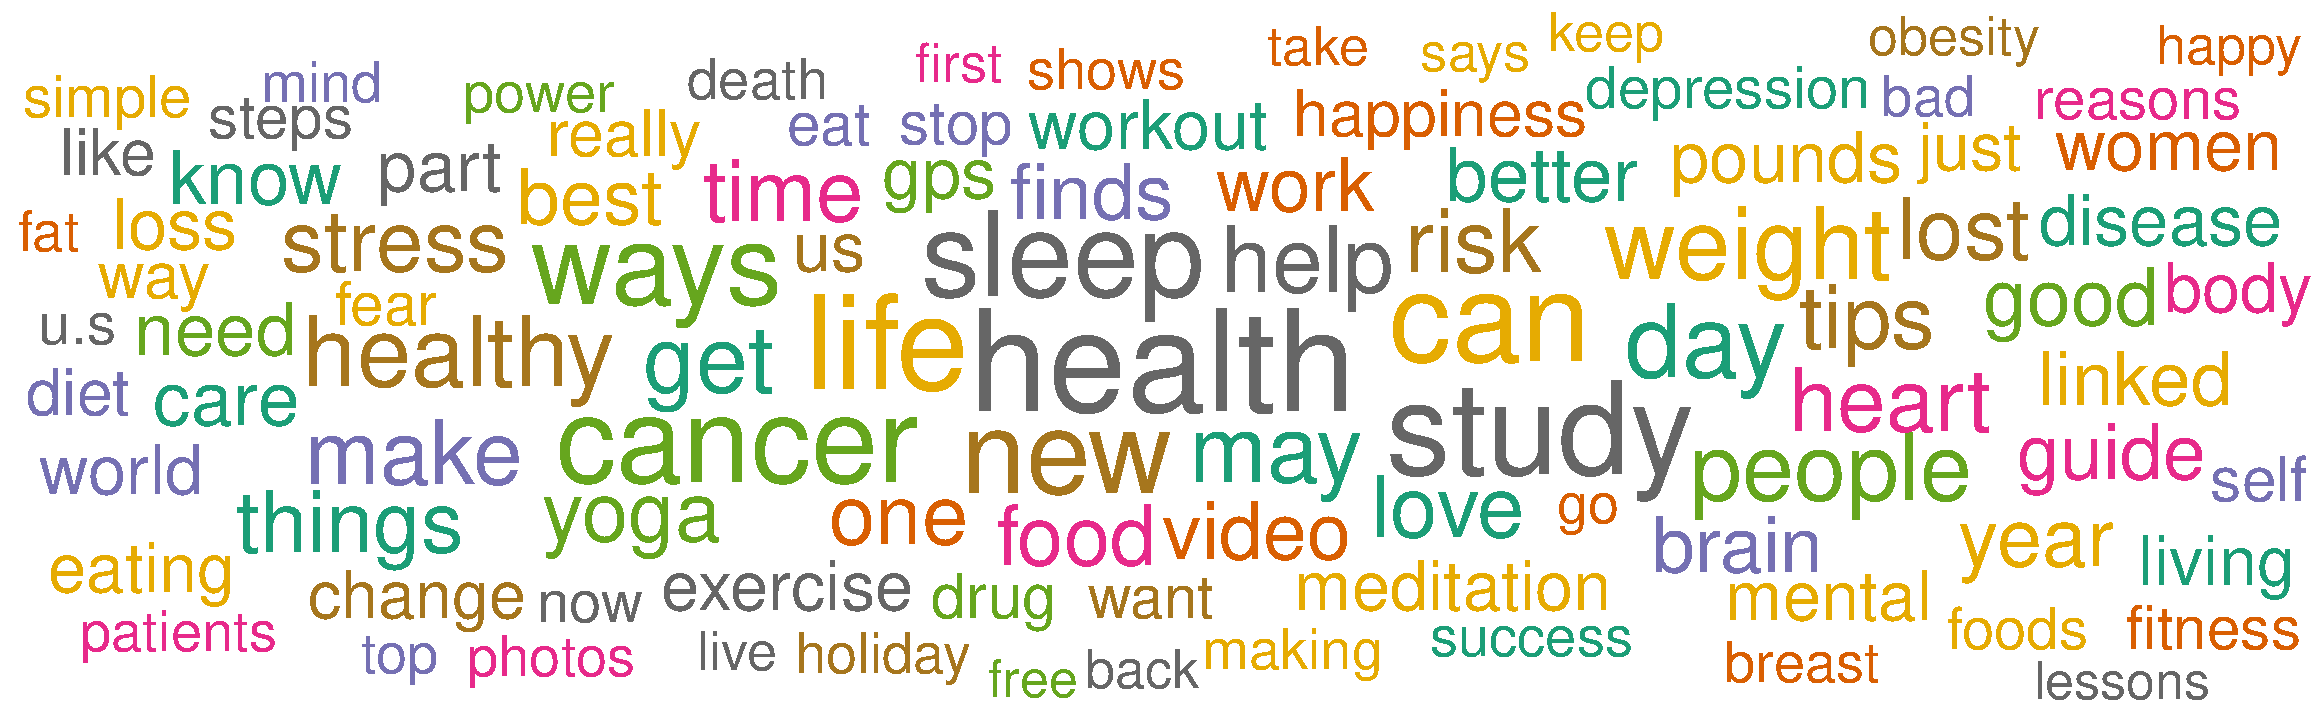
\includegraphics[width = \textwidth,  keepaspectratio]{Images/wordCloudWellness.pdf} 
\caption{\textit{Wordcloud} für die häufigsten 100 Wörter der Kategorie \textit{wellness \& healthy living}}
\label{abb:WordcloudWellness}
\end{figure}

In dieser Kategorie ist zu beobachten, dass oft über Schlaf, Yoga, Meditation und Sport geschrieben wird. Es werden aber auch Krankheiten wie Krebs (\say{cancer}), Übergewichtigkeit (\say{obesity}) und Diabetis angesprochen. \say{yoga}, \say{breast}, \say{diet} oder \say{pounds} könnten auch legitime Schlagwörter für die \say{women} Sparte sein. Genauso ist zu vermuten, dass die Wörter \say{eat}, \say{foods} und \say{healthy} ebenso in \say{food, drink \& taste} oft vorzufinden sind. Mit dem Blick auf die \textit{wordclouds} und auch in Anbetracht der Zusammenlegung der Kategorien in Kapitel \ref{kap:2_2Aend} fällt auf, dass es nicht immer einfach ist, die Kategorien nur über ihre häufigsten Schlagwörter auseinanderzuhalten. Auf die verschiedenen Möglichkeiten, wie die Schlagzeilen in ein numerisches Datenformat überführt werden können, wird in Kapitel \ref{kap:3.1Wordemb} detailiert eingegangen.
Nachdem nun der Datensatz ausführlich exploriert wurde, folgt im nächsten Unterabschnitt die Zielstellung dieser Thesis.


\subsection{Zielstellung} \label{Kap:Zielst}

Ziel dieser Arbeit soll es sein, verschiedene Algorithmen auf verschiedenen Arten der Repräsentation der Wörter miteinander zu vergleichen. Dabei liegt ein \textit{multiclass}-Klassifikations\-problem mit $32$ Klassen vor, bei der jede Beobachtung genau einer Klasse zugehörig ist. Die Zielvariable liegt im kategoriellen Format vor. Dabei soll für die Vorhersagen $f(x_i)$ der trainierten Modelle gelten, dass
\begin{center}
$f(x_i) = p_i = (p(c_1), ...., p(c_{32}))$ \hspace{2cm} , mit $\sum\limits_{i = 1}^{32} p(c_i) = 1 $,
\end{center}
dabei sind $p(c_j)$, $j = 1,...,32$ die modellierten Wahrscheinlichkeiten der Zugehörigkeit der Beobachtung $x_i$ zur Klasse $c_j$, die in Summe $1$ ergeben müssen. Die eindeutige prognostizierte Klasse $\hat{y}$ wird dann zugeordnet durch 
\begin{center}
    $\hat{y_i} =  \underset{c_1,...,c_{32}}{argmax}$ $p(c_j)$.
\end{center}

Bezüglich der Güte der Modelle soll dann mit den Gütemaßen aus Kapitel \ref{kap:guetemass} ein Vergleich erfolgen. Dabei ist nicht nur von Interesse, wie gut die Modelle insgesamt abschneiden, sondern auch ob manche Modelle bestimmte Kategorien trennschärfer identifizieren können und welche Gründe es dafür gibt. Des Weiteren soll analysiert werden, in welche Nachbarklassen die Beobachtungen bei einer Fehlklassifikation eingeordnet werden und ob diese inhaltlich nahe an der richtigen Kategorie sind. Eine weitere Untersuchungsfrage für die Modellgüte ist, inwiefern die Repräsentation der Wörter ausschlaggebend sind und welches Gewicht der verwendete Algorithmus dabei einnimmt.
Nun sollen im nächsten Abschnitt die statistischen Methoden beschrieben werden.
(todo: diesen Abschnitt im Laufe der Arbeit ergänzen)

\newpage



\section{Statistische Methoden}

Dieses Kapitel ist in $3$ Abschnitte unterteilt. Zuerst werden die zur Bewertung der Modelle herangezogenen Gütemaße beschrieben. Es folgt die Darlegung der verschiedenen Methoden zur numerischen Repräsentation von Wörtern. Zuletzt folgt die ausführliche Beschreibung der in dieser Arbeit benutzten \textit{machine-learning} Algorithmen.

\subsection{Gütemaße zur Evaluation der Modelle}\label{kap:guetemass}

Die Bewertung der Modelle erfolgt über verschiedene Kennzahlen. Einige davon werden unter Verwendung der \textit{confusion matrix} (oder auch Klassifikationsmatrix) berechnet. Wird das Modell auf die Testdaten angewandt und für jeden Datenpunkt eine Kategorie vorhergesagt, so stellt die in Tabelle \ref{tab:confusionMatrix} abgebildete Matrix die resultierenden Richtig- und Fehlklassifikationen für $C$ Klassen dar.

\begin{table}[ht]
\begin{center}
\begin{tabular}{|c|ccc|c|}
  \hline
 & \multicolumn{3}{|c|}{Prognostizierte Klasse} &  \\
Wahre Klasse & Kategorie $c_1$ & ...  & Kategorie $c_C$ & Zeilensumme  \\ 
  \hline
Kategorie $c_1$ & $h_{11}$ & $\hdots$ & $h_{1C}$ & $\sum_{j=1}^C h_{1j}$\\
$\vdots$ & $\vdots$ & $\ddots$ & $\vdots$ & $\vdots$ \\
Kategorie $c_C$ & $h_{C1}$ & $\hdots$ & $h_{CC}$ & $\sum_{j=1}^C h_{Cj}$\\
\hline
Spaltensumme & $\sum_{i=1}^C h_{i1}$ & $\vdots$ & $\sum_{i=1}^C h_{iC}$ & 
$N = \sum_{i=1}^C \sum_{j=1}^C h_{ij}$\\
   \hline
\end{tabular}

  \caption{Übersicht über eine \textit{confusion matrix}  für $C$  Klassen (vgl. \cite{backhaus}, S. 238)}  
  \label{tab:confusionMatrix}
\end{center}
\end{table}

Die absoluten Häufigkeiten $h_{ij}$ stehen für die Anzahl der Beobachtungen aus der wahren Klasse $i$, für die die Klasse $j$ prognostiziert wurde. Summiert man alle Einträge der Matrix, so erhält man die Anzahl der Beobachtungen $N$. Aus der \textit{confusion matrix} können folgende Größen identifiziert werden: Die \textit{true-positives} der Klasse $i$, $tp_i = h_{ii}$ sind alle Beobachtungen, die Klasse $i$ zugehörig sind und auch in selbige Klassifiziert wurden. Die Beobachtungen, die in Klasse $i$ klassifiziert wurden, aber einer anderen wahren Klasse zugehörig sind, bezeichnet man als \textit{false-positives} $fp_i = \sum_{j = 1}^C h_{ji} - h{ii}$. Als \textit{false-negatives} $tn_i = \sum_{j = 1}^C h_{ij} - h{ii}$ werden die Beobachtungen bezeichnet, die der Klasse $i$ zugehörig sind, aber in eine andere Kategorie falsch klassifiziert werden. Letztlich sind \textit{true-negatives} $fn_i = N - (fp_i + tn_i + \sum_{j \neq i} tp_j)$ die Datenpunkte, die nicht Kategorie $i$ angehören und für die auch nicht Klasse $i$ prognostiziert wird (vgl. \cite{sokolova}, S. 3). Unter Kenntnis der $4$ Häufigkeiten können nun verschiedene Gütemaße berechnet werden. 


Die \textit{accuracy} berechnet sich analog zur binären Klassifikation aus 
\[ accuracy = \frac{\sum_{i=1}^C tp_i}{N},  \]
ist also der Anteil der richtig klassifizierten Beobachtungen an allen Beobachtungen. Dieses Maß ist jedoch gerade bei unbalancierten Klassifikationsproblemen nicht ideal, da große Klassen stark favorisiert werden und ein Modell schon eine hohe Güte erzielen kann, indem es alle Beobachtungen der größten Klasse zuordnet (vgl. \cite{backhaus}, S.239). Es folgen die Maße \textit{precision}, \textit{recall} und darauf aufbauende Kennzahlen, welche bei unterschiedlichen Klassengrößen geeigneter sind. Es wird von einer hohen \textit{precision} der Klasse $i$ gesprochen, wenn nach Prognose in Klasse $i$ ein hoher Anteil dieser Beobachtungen auch tatsächlich aus derselben Kategorie stammt. Wiederum hat das Modell bezüglich Klasse $i$ einen hohen \textit{recall}, falls von den Beobachtungen der wahren Klasse $i$ auch ein hoher Anteil in Klasse $i$ eingeordnet wird.
In der \textit{multiclass}-Klassifikation kann ein Gütemaß für das komplette Modell über \textit{micro-averaging} (mit $\mu$ indiziert) oder \textit{macro-averaging} (mit $M$ indiziert) über alle Klassen berechnet werden. Es sind dann 
\[ precision_{\mu} = \frac{\sum_{i = 1}^C tp_i}{\sum_{i = 1}^C (tp_i + fp_i)}, \hspace{1cm} recall_{\mu} = \frac{\sum_{i = 1}^C tp_i}{\sum_{i = 1}^C (tp_i + fn_i)},\]
\[ precision_M = \frac{\sum_{i = 1}^C \frac{tp_i}{tp_i + fp_i} }{C}, \hspace{1cm} recall_M = \frac{\sum_{i = 1}^C \frac{tp_i}{tp_i + fn_i} }{C}\]
die Gütemaße für das gesamte Modell. Ein Maß, dass \textit{precision} und \textit{recall} kombiniert ist der \textit{fscore}. Mit der unterschiedlichen Durchschnittsbildung ergeben sich
\[ fscore_{\mu}^{(\beta)} = \frac{(\beta^2+1) precision_{\mu} recall_{\mu}}{\beta^2 precision_{\mu}+ recall_{\mu}}, \hspace{1cm} fscore_{M}^{(\beta)} = \frac{(\beta^2+1) precision_{M} recall_{M}}{\beta^2 precision_{M}+ recall_{M}} . \]


Hierbei ist anzumerken, dass $fscore_{\mu}^{(\beta)}$ Klassen mit vielen Beobachtungen in der Güte begünstigt während für $fscore_M^{(\beta)}$ alle Kategorien gleich wichtig sind  (vgl. \cite{sokolova}, S.3ff). Der Parameter $\beta$ gibt in den Formeln an, was für ein Gewicht \textit{recall} im Verhältnis zu \textit{precision} einnimmt.
Wie bei dem \textit{f1-score} Maß einer binären Klassifikation wird in dieser Arbeit $\beta = 1$ verwendet. \textit{recall} und \textit{precision} besitzen also identische Wichtigkeit. \\
Bei Betrachtung des Nenners in der Berechnung von $precision_{\mu}$ und $recall_{\mu}$ fällt auf, dass in beiden Fällen durch die gesamte Summe der \textit{Confusion Matrix} geteilt wird. Diese Summe entspricht dem Nenner $N$ bei der Berechnung der $accuracy$. Ist nun auch $\beta = 1$, so gilt 
\[precision_{\mu} =  recall_{\mu} =  fscore_{\mu}^{(1)} = accuracy.\]

Für eine beispielhafte Erklärung dieses Sachverhaltes sei auf \cite{towards1} verwiesen. Aus diesem Grund wird statt der mit \textit{micro-averaging} berechneten Gütemaße in der statistischen Auswertung in Kapitel \ref{Kap:statAus} die $accuracy$ verwendet.\\

Ein weiteres Maß, um die Güte eines Multiklassifikationsproblems zu bewerten ist die gemittelte \textit{categorical cross entropy}. Diese berechnet sich aus

\[ CE = - \frac{1}{N}\sum_{i=1}^N \sum_{j = 1}^C y_{ij} log(p_i(c_j)) \]

(vgl. \cite{murphy}, S.571) wobei $y_{ij} \in \{0,1\}$ \hspace{0.2cm} $\forall i, j = 1,...,N$ indiziert, ob die Beobachtung $i$ der wahren Klasse $j$ zugehörig ist und $p_i(c_j)$ die vom Modell vorgegebene Wahrscheinlichkeit ist, dass Beobachtung $i$ zu Klasse $j$ gehört. Da $y_{ij}$ immer $0$ für alle falschen vorhergesagten Klassen ist, entspricht $CE$ dem negativen Mittelwert der logarithmierten Wahrscheinlichkeiten der wahren Klassen über alle Beobachtungen. So wird eine geschätzte Wahrscheinlichkeit nahe $0$ für die wahre Klasse stark bestraft und eine hohe Wahrscheinlichkeit trotz einer Fehlklassifikation weniger bestraft. Je sicherer sich das Modell für die wahren Kategorien ist, desto niedrigere Werte wird dieses Gütemaß annehmen (vgl. \cite{proMachine}, S. 72). 
Dabei gilt es die \textit{cross entropy} zu minimieren. Sie nimmt ihr Minimum bei $0$ im Idealfall an, wenn für alle Beobachtungen eine Wahrscheinlichkeit von $1$ für die wahre Klasse prognostiziert wird. Die $CE$ wird oft als Verlustfunktion für die Modellanpassung auf den Trainingsdaten verwendet, wie zum Beispiel bei \textit{xgBoost} und den \textit{deep learning} Algorithmen aus Kapitel \ref{kap:neuralNets}.\\
\\
Die in diesem Abschnitt beschriebenen Maße können sowohl auf den Trainingsdaten als auch auf den  Validierungs- und Testdaten berechnet werden. Ein Vergleich der Modelle in der Vorauswahl in Abschnitt \ref{kap:preselection} erfolgt über die Evaluation auf den Validierungsdaten. Dabei werden die Maße $accuracy$, $CE$, und $fscore_M^{(1)}$ genutzt.
Bei dem Vergleich der finalen Modelle in Kapitel \ref{kap:evalFinal} erfolgt die Auswertung der Performanzmaße auf den ungesehenen Testdaten. (todo: aufführen was noch alles verwendet wurde).


\subsection{Methoden zur numerischen Repräsentation der Wörter} \label{kap:3.1Wordemb}

Das Extrahieren von Informationen aus Texten ist keine triviale Aufgabe, für die es viele Methoden gibt. In diesem Abschnitt werden einige Methoden aufgezählt, die in dieser Thesis zum Einsatz kommen.


\subsubsection{\textit{bag-of-words} und \textit{term frequency inverse document frequency}} \label{Kap:Tfidf}

Bei diesen Methoden wird zuerst für den gesamten Textkorpus ein Vokabular gebildet, das für jedes vorkommende Wort die absolute Häufigkeit des Vorkommens sowie die Anzahl der Dokumente (ein Dokument ist ein Datenpunkt, also eine Schlagzeile) enthält, in der das Wort vorkommt. Aus diesem Vokabular wird anschließend die Matrix $dtm$ (\textit{document-term-matrix}) geformt, die für jede der $N$ Beobachtungen eine Zeile und für jede der $V$ Wörter im Vokabular eine Spalte enthält. Die Einträge der Matrix bestehen aus Werten, die das Aufkommen der Wörter beschreiben. Im simplen \textit{bag-of-words} (kurz: \textit{bow}) Ansatz ist $dtm_{ij} = f_{d_i t_j}$ die Anzahl von Wort $t_j$ in Dokument $d_i$ (vgl. \cite{deepEssentials} S. 117f). Es gibt einige Wörter wie \textit{the} oder \textit{and}, die häufig vorkommen aber eventuell nicht wichtig sind. Diese \textit{stopwords} können für die \textit{bow} Methode entfernt werden. Dies muss aber nicht erfolgen, da manche \textit{stopwords} in einen Kategorien häufiger vorkommen können als in anderen.
Im \textit{bow} wird nur gezählt, wie oft ein Wort absolut vorkommt, dabei wird aber nicht berücksichtigt, dass manche Wörter in einigen Dokumenten eine höhere Bedeutung haben können als in anderen. \\

Ein Ansatz, der diese Problematik berücksichtigt ist \textit{term frequency inverse document frequency} (kurz: \textit{tf-idf}). Hierbei werden die Einträge $dtm_{ij}$ bei häufig benutzten Ausdrücken verringert und erhöht für Wörter, die insgesamt selten benutzt werden (vlg. \cite{textMiningR} S.29). Die \textit{tf-idf} für das Dokument $d_i$ und das Wort $t_j$ berechnet sich aus 
\[tfidf(d_i, t_j) = tf(d_i,t_j) \cdot idf(t_j) . \]
Sowohl für die \textit{term-frequency} $tf$ als auch für die \textit{inverse-document-frequency} $idf$ gibt es verschiedene Möglichkeiten zur Berechnung, wobei in dieser Thesis folgende Formeln genutzt werden.
Die \textit{augmented-term-frequency}

\[tf(d_i,t_j) = 0.5 +  0.5 \cdot \frac{f_{d_i t_j}}{max \{ f_{d_i t_j'}: t_j' \in d_i \}} \].

berücksichtigt eine Verzerrung bei längeren Dokumenten, indem durch das Maximum der vorkommenden Wörter in dem Dokument dividiert wird. Der Summand $0.5$ und der Multiplikator $0.5$ dienen der Normalisierung. Für die \textit{inverse document frequency} ist der Quotient zwischen der Anzahl der Dokumente $N$ im Korpus und der Anzahl der Dokumente, die das Wort enthalten, ein geeignetes Maß (vgl. \cite{deepEssentials} S. 118):

\[idf(t_j) = log(\frac{N}{\# \{d_i: t_j \in d_i \}}) .\]

Die Umsetzung im Programmiercode erfolgte mit dem \texttt{R}- Paket \texttt{text2vec} (\cite{text2vec}) und die beiden \textit{Embeddings} werden ab hier mit \textit{BOW} und \textit{TFIDF} referenziert.\\

Unter Nutzung von sowohl \textit{bow} als auch \textit{tfidf} für die Repräsentation von Wörtern vernachlässigt man die Reihenfolge in den Dokumenten (vgl. \cite{deepEssentials} S. 117). 
Die nachfolgend beschriebenen Methoden berücksichtigen hingegen die Reihenfolge der Wörter in einem Satz.


\subsubsection{\textit{GloVe: Global vectors for representation of words}} \label{Kap:Glove}

Eine weitere Methode zur numerischen Repräsenation von Texten sind \textit{word embeddings}, bei denen Wörter zu Vektoren fester Länge mit numerischen Werten kodiert werden. Mittlerweile haben sich \textit{word embeddings} als präferierte Methode für alle Bereiche der Sprachverarbeitung im \textit{machine-learning} durchgesetzt. Die beiden bekanntesten Methoden um \textit{word embeddings} zu generieren sind \textit{word2vec} und \textit{GloVe} (vgl. \cite{keras}, S. 139). Obwohl \textit{word2vec} auf dem Lernen durch ein neuronales Netz basiert und \textit{GloVe} auf der Zählung des Vorkommens von Wörtern im Kontext aufbaut, sind die beiden Verfahren von der grundsätzlichen Herangehensweise und den Resultaten ähnlich. Beide Methoden konstruieren einen Vektorraum, in dem die Position eines Worts durch den Kontext bestimmt wird, in dem das Wort im Textkorpus auftritt.
\textit{GloVe} liefert im Vergleich zu \textit{word2vec} generell etwas bessere Resultate und ist mit Paralellisierung schneller zu berechnen (vgl. \cite{keras}, S. 156). Aus diesen Gründen wird in dieser Thesis \textit{GloVe} verwendet und im Folgenden beschrieben. \\
Die Methode nutzt ein unüberwachtes Lernen zur Konstruktion der Vektoren. Zuerst wird eine Matrix $R$ konstruiert, die so viele Zeilen enthält, wie das Vokabular Wörter besitzt. Die Spalten stehen ebenso für die Wörter des Vokabulars, allerdings als Kontext verstanden. In den Einträgen der Matrix stehen nun die Häufigkeit des Vorkommens der Wörter (Zeilen) im jeweiligen Kontext (Spalten). Ob ein Wort im Kontext vorkommt, ist so zu verstehen, dass es in einem vom Anwender wählbaren Fensterbereich um das Kontextwort enthalten ist. Zur Verdeutlichung sei folgender Satz gegeben: \textit{these quotes from kids are hilarious, adorable and oddly insightful}. So kommt für einen symmetrischen Bereich von $2$ dass Wort \textit{hilarious} im Kontext von \textit{kids} einmal vor, wobei \textit{insightful} nicht im Kontext von \textit{kids} vorkommt. 
Die Matrix $R$ wird nun in das Produkt aus 2 Matrizen $P$ und $Q$ zerlegt, die multipliziert eine fast identische Matrix $\Tilde{R}$ ergeben:

\begin{equation*}
\underset{N \times N}{R} = \underset{N \times F}{P} \cdot \underset{F \times N}{Q} \approx  \underset{N \times N}{\Tilde{R}} 
\end{equation*}

Die Matrix $P$ mit Dimension $N \times F$ ergibt multipliziert mit $Q$ mit Dimensionen $F \times N$ wieder eine $N \times N$ Matrix. Nun werden sowohl $P$ als auch $Q$ mit zufälligen Werten initiiert und die Matrix $\Tilde{R}$ berechnet. Mithilfe des stochastischen Gradienten-Abstieg (mehr dazu in Kapitel \ref{kap:neuralNets}) wird nun der Inhalt von $P$ und $Q$ verändert, mit dem Ziel die Summe aller Einträge der Differenz von $\Tilde{R}$ und $R$ zu minimieren. Dies ist ein numerischer iterativer Prozess, der wiederholt wird, bis der Fehler eine vorgegebene untere Grenze erreicht. Die Matrix $P$ enthält nun die gewünschten \textit{word-embeddings} (vgl. \cite{keras}, S. 155f). Für eine detailierte Beschreibung der Methode sei auf \cite{glovePaper} verwiesen. Die Dimension $F$ der Wort-Vektoren muss vom Anwender festgelegt werden. Es ist möglich diese Vektoren auf dem vorliegenden Trainingsdatensatz zu trainieren, wenn der Textkorpus groß genug ist. In dem Fall des \textit{news category dataset} mit $200847$ ist dies durchaus plausibel. Das Trainieren der Vektoren erfolgte mit dem \texttt{R}-Paket \texttt{text2vec} (\cite{text2vec}) unter Verwendung der Parameter $skip\_grams\_window = 5$ für den symmetrischen Bereich des Kontextworts und die Dimension der Vektoren von $F = word\_vectors\_size = 50$. Dieses \textit{Embedding} wird mit dem Kürzel \textit{GloVe unsup. 50D} referenziert. \\
Eine Alternative zum Training der \textit{word-embeddings} auf dem vorliegenden Textkorpus ist der Griff zu einem der vortrainierten Datensätze, die von \cite{gloveOnline} zur Verfügung gestellt worden sind. Diese Vektoren wurden auf massiven Datenmengen trainiert. Für diese Arbeit wurden 2 Datensätze mit vor-trainierten Wortvektoren des \textit{GloVe} Projekts genutzt: Ein auf Wikipedia mit $6$ Milliarden Dokumenten trainierter Datensatz mit einer Länge der Vektoren von $F = 50$ (\cite{gloveWiki}) und ein auf $42$ Milliarden aus verschiedensten Quellen des Internets stammenden Textdokumenten mit $F = 300$ Dimensionen (\cite{gloveCommon}). Die beiden vortrainierten \textit{Embeddings} werden in Kapitel \ref{Kap:statAus} mit \textit{GloVe 50D} und \textit{GloVe 300D} referenziert.\\

Ob nun vor-trainierte \textit{word embeddings} genutzt werden oder die Vektoren auf dem Trainingsdatensatz gelernt werden, es stellt sich die Frage, wie genau die Datenpunkte geformt werden, sodass ein \textit{machine learning} Modell immer Eingangswerte derselben Dimension erwarten kann. Nun ist unter der Annahme, dass eine Beobachtung immer aus einer Aneinanderreihung von Wörtern besteht, jeder durch Wort-Vektoren repräsentierter Datenpunkt $x_i$ bereits eine zweidimensionale Matrix mit Dimensionen $F \times  W_i$. $W_i$ steht für die Anzahl Wörter im Satz des Datenpunktes $x_i$ und $F$ ist die Anzahl der Wort-Vektoren. Damit die kodierten Datenpunkte nun jeweils die gleiche Dimension besitzen um zu einem dreidimensionalen Trainings-Array geformt werden zu können, soll $W_i$ immer gleich gewählt werden. Hier wird als Konstante $W_{max}$ die Anzahl Wörter gewählt, die $99.9$ Prozent der News Schlagzeilen im Trainingsset nicht überschreiten. Für jede Schlagzeile, die weniger Wörter als $W_{max}$ enthält, wird die Matrix für die fehlenden Wörter mit Nullen aufgefüllt (dies wird \textit{padding} genannt). Wäre $W_{max}$ die maximale Anzahl von Wörtern, die die größte Schlagzeile enthält, so würde durch das Auffüllen von vielen Nullen nur unnötig Speicherplatz verbraucht werden. \\

Allgemein haben die resultierenden Vektoren einige nützliche Eigenschaften. Als Ähnlichkeits\-maß zwischen 2 Vektoren kann das Kreuzprodukt genutzt werden. Wörter, die einander ähnlich sind, sind auch im $F$-dimensionalen Vektorraum nahe beieinander angeordnet. Falls die \textit{word-embeddings} auf großen Datenmengen trainiert worden sind, können die Vektoren sogar semantische Beziehungen repräsentieren. So kann beispielsweise \textit{walking} zu \textit{walked} dieselbe Beziehung haben wie \textit{swimming} zu \textit{swam}. Addiert oder subtrahiert man Wort-Vektoren, so können sogar Gleichungen der Form $king - man + women \approx queen$, oder $berlin - germany + france \approx paris$ zustande kommen (vlg. \cite{deepEssentials}, S. 122).

\subsubsection{Summe von Wort-Vektoren}

Die im vorherigen Abschnitt \ref{Kap:Glove} beschriebenen \textit{word-embeddings} bilden bei Sätzen immer eine zweidimensionale Matrix pro Datenpunkt. Es ist aber auch eine Dimensionsreduktion möglich indem die Vektoren unter bestimmten Regularisierungen summiert werden oder Differenzen gebildet werden. \cite{sumsWords}, S. 13 zeigen, dass die Summe der Word-Vektoren mit $L1$ Regularisierung eine gute Repräsentation der Sätze ist und gute Resultate liefert. Dies ist definiert als

\[SOW_{L1} = \frac{\sum_{i=1}^{W_{max}} \Vec{w_i}}{\| \sum_{i=1}^{W_{max}}  \vec{w_i} \|} \]
(\cite{sumsWords}, S. 5). Die $L1$ Norm skaliert die Einträge der $\Vec{w_i}$ so, dass die Summe aller Einträge $1$ entspricht. Es wird bis $W_{max}$ summiert, da das in Kapitel \ref{Kap:Glove} erläuterte \textit{padding} dafür sorgt, dass jede Schlagzeile mit genau $W_{max}$ Vektoren der Länge $F$ repräsentiert werden. Aufgrund der Auffüllung mit Nullen für fehlende Wörter beeinflusst dies den Summand nicht.
Jeder Datenpunkt wird zusammenfassend als Vektor mit $F$ Einträgen dargestellt, die die Bedeutung des dahinterstehenden Satzes im $F$ dimensionalen Raum repräsentieren. Die entsprechenden Summen der \textit{Embeddings} aus \ref{Kap:Glove} werden in der Vorauswahl in Kapitel \ref{kap:preselection} als \textit{SOW GloVe unsup. 50D}, \textit{SOW GloVe 50D} und \textit{SOW Glove 300D} bezeichnet.


\subsubsection{Sequentielle Darstellung} \label{Kap:Seq}

Eine weitere Möglichkeit, Sätze und Wörter zu repräsentieren ist als Sequenz von Indices. So bekommt jedes Wort eine natürliche Zahl aus dem Vokabular zugeordnet. Durch die Aneinanderreihung dieser Indices wird ein Satz als Sequenz von natürlichen Zahlen dargestellt. Die resultierende Datenmatrix hat also die Dimensionen $N \times W_{max}$, wobei $W_{max}$ analog wie in Kapitel \ref{Kap:Glove} gewählt wird. Diese kann als Trainingsdatensatz für ein klassisches \textit{machine-learning} Modell wie \textit{random Forest} (Kapitel \ref{kap:RF}), oder als Input für neuronale Netze wie \textit{CNN} (Kapitel \ref{kap:CNN}) oder \textit{LSTM} (Kapitel \ref{kap:LSTM}) dienen. Eine \textit{embedding} Eingangsschicht im neuronalen Netz lernt jeden Index dann zu einem Wort-Vektor einer vorgegebenen Größe $F$ und jeder Datenpunkt wird intern zu einer Matrix der Dimension $F \times W_{max}$ während des Trainieren des Netzes geformt. Das Bilden der \textit{word embeddings} geschieht in diesem Fall durch überwachtes Lernen und nicht durch unüberwachtes Lernen wie bei \textit{GloVe} in Kapitel \ref{Kap:Glove} (vgl. \cite{keras}, S.159f).\\
Die Erstellung der Wort-Sequenzen erfolgte in \texttt{R} mit dem Paket \texttt{keras} (\cite{kerasR}). In Kapitel \ref{kap:preselection} ist diese Art der Repräsentation der Wörter mit dem Kürzel \textit{Sequence} benannt. \\


\subsection{\textit{machine learning} Modelle}\label{kap:machineLearning}

\subsubsection{Extreme Gradient Boosting}\label{kap:XG}
\subsubsection{Random Forest}\label{kap:RF}

\subsection{Neuronale Netze} \label{kap:neuralNets}

Dieses Unterkapitel gibt eine Einführung in das Gebiet der neuronalen Netze und die in dieser Arbeit verwendeten Architekturen. Beginnend mit dem \textit{multi-layer-perceptron} Netz werden die allgemeinen Aspekte und Komponenten des \textit{deep learnings} erläutert. Daran anknüpfend werden mit dem Fokus auf \textit{natural language processing} (die Verarbeitung von Textdaten, kurz \textit{NLP}) das \textit{convolutional neural net} (kurz \textit{CNN}) und das \textit{long-short-term-memory neural net} (kurz \textit{LSTM}) beschrieben. Die Implementierung der Netzarchitekturen im Programmiercode erfolgte mit dem \texttt{R}-Paket \texttt{keras} (\cite{kerasR}).


\subsubsection{Multi-Layer-Perceptron Neural Net}

Dieser Abschnitt basiert größtenteils auf \cite{deepEssentials}, S.60-71 und S.214-230.
Das \textit{Multi-Layer-Perceptron} (kurz \textit{MLP}) ist die einfachste Form eines neuronalen Netzes. Anhand des \textit{MLP} wird im Folgenden beschrieben, wie die Struktur und die Bestandteile eines neuronalen Netzes aussehen, wie es die Gewichtsparameter lernt und welche Komponenten besonders wichtig sind für die erfolgreiche Anwendung. Abbildung \ref{abb:MLPScreen} zeigt die klassische Struktur eines \textit{MLP}:


\begin{figure}[!ht]
\begin{center}
\includegraphics[width = 10cm,  keepaspectratio]{Images/MLPScreenDeepLearningEssentials.PNG}
\caption{\textit{fully-connected feed-forward} Netz mit 2 Zwischenschichten (\cite{deepEssentials}, S. 60)}
\label{abb:MLPScreen}
\end{center}
\end{figure}

In der Abbildung \ref{abb:MLPScreen} ist zu sehen, dass das Netz in verschiedenen Schichten organisiert ist, die jeweils aus Neuronen (auch Knoten oder Zellen genannt) bestehen. Die Eingangsschicht (\textit{input layer}) besteht aus den als numerischen Werten kodierten Trainingsdaten und enthält entsprechend viele Neuronen. Darauf folgen mehrere Zwischenschichten (\textit{hidden layer}. Die Zwischenschichten enthalten jeweils eine vom Nutzer wählbare Anzahl von Neuronen. Die Ausgangsschicht (\textit{output layer}) schließt das Netz ab. Wie viele Knoten die Ausgangsschicht enthält, ist abhängig von der Problemstellung. Im Falle einer Klassifikation mit $C$ Klassen enthält es ebenso viele Knoten. Nun bedeutet \textit{fully-connected}, dass jedes Neuron mit allen Neuronen aus der vorherigen und nachfolgenden Schicht verbunden ist. Bei einem \textit{feed-forward} Netz werden nur Verbindungslinien in eine Richtung zugelassen und zwar von Eingangs- bis Ausgangsschicht. Die Verbindungslinien werden durch Gewichte repräsentiert, die den Einfluss des Eingangsneuron auf das Ausgangsneuron beschreiben. Seien $a_1^{(k-1)},..., a_{m^{(k-1)}}^{(k-1)}$ die Ausgangssignale der $k-1$-ten Zwischenschicht und $a_{1}^{(k)},..., a_{m^{(k)}}^{(k)}$ die Neuronen der $k$-ten Zwischenschicht. $m^{(k)}$ bezeichnet hierbei die Anzahl Neuronen in der $k$-ten Zwischenschicht. 
Das Gewicht $w_{i_l}^{(k)}$ gehört zur Verbindungslinie von Knoten $i$ der $k-1$-ten Zwischenschicht mit Knoten $l$ der $k$-ten Zwischenschicht. Das Signal, dass das $l$-te Neuron der $k$-ten Zwischenschicht $a_{l}^{(k)}$ erreicht, berechnet sich aus der gewichteten Summe der Eingangsdaten und einem \textit{bias}, auf die dann eine Aktivierungsfunktion $\sigma$ angewandt wird:

\[ a_{l}^{(k)} = \sigma (b_l + \sum_{i=1}^{m^{(k-1)}} w_{il}^{(k)} a_{i}^{(k-1)}).\]

Der \textit{bias} $b_l$ ist ein weiterer Parameter, der im Laufe des Trainings des Netzes gelernt wird.
Für die erste Zwischenschicht und die Eingangsschicht berechnen sich Signale analog indem die Eingangssignale $a_{1}^{(k-1)},..., a_{m^{(k-1)}}^{(k-1)}$ durch die Einträge des Datenvektors $x_1, ..., x_F$ ersetzt werden, mit $F$ der Anzahl der Variablen oder der Dimension des Wort-Vektors. Die Aktivierungsfunktion $\sigma$ transformiert die gewichtete Summe dann anschließend und bestimmt wie hoch das finale Signal ist. Jede Schicht außer der Eingangsschicht besitzt eine solche Aktivierungsfunktion. Sie sollte differenzierbar sein, da das Netzwerk im Prozess des Lernens Gradienten berechnet. Dieser Aspekt wird später detailliert erläutert. Es existiert eine Vielzahl an Aktivierungsfunktionen. Es werden im Folgenden Aktivierungsfunktionen vorgestellt, die in dieser Arbeit genutzt werden (vgl. \cite{deepEssentials}, S.62-65). 

Die \textit{sigmoid} Aktivierungsfunktion bildet die Urmenge in das Intervall $\left[0, 1\right]$ ab. Sei $x \in \mathbb{R}$ ein Input, dann ist 

\[\sigma(x) =  \frac{1}{1+ e^{-x}}.\]

Eine Funktion, die die Urmenge in das Intervall $\left[-1, 1\right]$ abbildet, ist der \textit{tangens hyperbolicus}, der wie folgt definiert ist:

\[tanh(x) =  \frac{1- e^{-2x}}{1+ e^{-2x}}.\]


Die Konvergenz der Parameter erfolgt schneller als unter der Nutzung von einer \textit{sigmoid} Aktivierung. Dennoch leidet $tanh$ wie die \textit{sigmoid} Funktion unter dem \textit{vanishing gradient} Problem, weshalb in der Praxis die \textit{rectified linear unit} (kurz \textit{relu}) genutzt wird. \textit{sigmoid} und \textit{tanh} finden in dieser Thesis ausschließlich Anwendung bei den in Kapitel \ref{kap:LSTM} beschriebenen \textit{long-short-term-memory neural networks}. Die \textit{relu} Funktion ist wie folgt definiert:

\[relu(x) = 
\begin{cases}
max(0,x), & x >= 0 \\
0, & x <0
\end{cases}{}
.\]

Es wurde gezeigt, dass im Lernprozess die Konvergenz der Parameter unter Nutzung von \textit{relu} bis zu 6-Mal schneller erreicht werden kann. Außerdem benötigt ihre Berechnung weniger Rechenleistung als klassische Aktivierungsfunktionen. \textit{relu} wird heutzutage aus diesen Gründen in den meisten neuronalen Netzen in den Zwischenschichten verwendet (vgl. \cite{deepEssentials}, S. 64). Für die Ausgangsschicht muss eine Aktivierungsfunktion gewählt werden, die Werte im Intervall $\left[0, 1\right]$ annimmt und dabei gleichzeitig eine Art Wahrscheinlichkeit modelliert. Hierbei wird im Klassifikationsfall zur \textit{softmax} Aktivierungsfunktion gegriffen. 

\[p(y = j |z_j) = \phi(z_j) = \frac{e^{z_j}}{\sum_j^C z_j} \]

Hierbei bezeichnet $z_j$ das Eingangssignal in das Neuron der $j$-ten Klasse und $y$ die wahre Klasse. $\phi$ transformiert und normiert die Ausgangssignale für jedes der $C$ Neuronen in der Ausgangsschicht und modelliert unter der Bedingung $z_j$, für jede der Klassen $j = 1,..., C$ eine Wahrscheinlichkeit $p(y=j|z_j) \in \left[0, 1\right]$. Insgesamt ergibt sich $\sum_{j = 1}^C \phi(z_j) = 1$. Für die in dieser Arbeit verwendeten neuronalen Netze wird jeweils eine Ausgangsschicht mit $n = 32$ Knoten gewählt und die \textit{softmax} Aktivierungsfunktion zur Transformation der Eingangssignale genutzt (vgl. \cite{deepEssentials}, S. 65).\\
\\
Nachdem nun die grundlegende Architektur des Netzwerkes und die Aktivierungsfunktionen erläutert wurden, wird nun der Lernprozess durch den Gradientenabstieg und die damit verbundene Anpassung der Gewichte beschrieben. Die Optimierung des Netzwerkes geht insofern von statten, dass die Funktion $f(x)$ bezüglich einer Verlustfunktion minimiert wird, indem $x$ geändert wird. $x$ ist hier das mathematische Resultat der \textit{forward propagation}. Dies ist der Prozess, bei dem die Input Daten durch das Netz geschleust werden und wird später noch beispielhaft erklärt.
Der Wert, der $f$ minimiert, wird notiert als 

\[\bm{x}^\ast = argmin f(x)\]

$\bm{x}^\ast$ ist der resultierende Parametervektor.
Seien $x, y := f(x) \in \mathbb{R}$, so ist $f'(x) = \frac{\mathop{dx}}{\mathop{dy}}$ die Steigung in $x$ und gibt an, in was für einer Änderung $f(x)$ bei einer kleinen Änderung von $x$ resultiert. Unter Kenntnis von $f'(x)$ kann $f(x)$ schrittweise durch eine Änderung von $x$ in die Gegenrichtung der Ableitung minimiert werden. Diese Methode ist bekannt als Gradientenabstieg. Ist $f'(x) = 0$, so handelt es sich entweder um ein Minimum, Maximum oder einen Sattelpunkt. Ziel des Gradientenabstieg ist es, ein globales Minimum zu finden. Es ist möglich, dass die Funktion auch einige lokale Minima besitzt, in denen $f(x)$ in einem Teil des Wertebereichs ein Minima annimmt, aber eben nicht den kleinsten Wert im gesamten Wertebereich. Das Vorliegen von mehreren Sattelpunkten und lokalen Minima macht die Optimierung sehr schwierig, besonders, da es sich in der Praxis um multidimensionale Optimierungen handelt. Oft werden solche Lösungen akzeptiert, die nicht global minimal sind, aber einen signifikant niedrigen Wert der Verlustfunktion aufweisen. Abbildung \ref{abb:MinimaSearch} zeigt eine beispielhafte Darstellung einer eindimensionalen Verlustfunktion mit verschiedenen Minima und Sattelpunkten.

\begin{figure}[!ht]
\begin{center}
\includegraphics[width = 10cm,  keepaspectratio]{Images/MinimaSearch_DeepL.PNG}
\caption{\textit{Darstellung von lokalen und globalen Minima sowie Sattelpunkten bei der Optimierung einer eindimensionalen Funktion (\cite{deepL}, S. 85)}}
\label{abb:MinimaSearch}
\end{center}
\end{figure}

Die Verlustfunktion ist in Abhängigkeit des Parameter-Vektors $\bm{x}^\ast$ üblicherweise nicht-linear und nicht-konvex, wie beispielsweise in Abbildung \ref{abb:MinimaSearch} zu sehen ist. Oft ist es möglich, dass der Gradientenabstieg in einem ungenügenden lokalen Minimum endet. Verschiedene Optimierungsalgorithmen versuchen dieses Problem zu lösen und werden im weiteren Verlauf dieses Kapitels beschrieben.\\

Ist $\bm{x} = (x_1, ..., x_l) \in \mathbb{R}^l$, so werden partielle Ableitungen $\frac{\partial}{\partial x_i} f(\bm{x})$ gebildet, die die Richtungsänderung von $f$ darstellt, wenn nur $x_i$ in $\bm{x}$ modifiziert wird. Der Vektor aller partiellen Ableitungen $(\frac{\partial f(\bm{x})}{\partial x_i}, \dots, \frac{\partial f(\bm{x})}{\partial x_l)})$ ist der Gradient von $f$ und wird notiert als $\nabla_{\bm{x}} f(\bm{x})$ (vgl. \cite{deepL}, S.82 ff).\\

Nun soll die Methode des Gradientenabstiegs an einem einfachen Beispiel erläutert werden. In einem Netzwerk mit 2 Zwischenschichten sei $(\bm{x_0}, \bm{y})$ der Eingangsvektor und der Vektor der dazugehörigen Zielvariable sowie $(\bm{w_1}, \bm{b_1})$, $(\bm{w_2}, \bm{b_2})$ die Vektoren der Gewichte und \textit{bias} der Zwischenschichten. Der erste Schritt ist die Initialisierung der Gewichte und der \textit{bias} Parameter. Die Gewichte werden mit kleinen zufällige Werten initialisiert und die \textit{bias} Parameter entweder auf $0$ gesetzt oder auch mit kleinen positiven Zufallszahlen belegt (vgl. \cite{deepL}, S. 177). Als nächstes werden die Eingangsvektoren im Rahmen der \textit{forward-propagation} vorwärts durch das Netz geleitet. Die Berechnung erfolgt sukzessive mit
\begin{align*}
    \bm{z_1} &= \bm{x_0} \cdot \bm{w_1} + \bm{b_1} \\
    \bm{a_1} &= \sigma(\bm{z_1}) \\
    \bm{z_2} &= \bm{a_1} \cdot \bm{w_2} + \bm{b_2} \\
    \bm{a_2} &= \sigma (\bm{z_2})
\end{align*}{}
$\bm{z_1}, \bm{z_2}$ sind die Vektoren, die in den Zwischenschichten eintreffen, $\bm{a_1}, \bm{a_2}$ die Signale, die die Neuronen der Zwischenschichten wieder verlassen und $\sigma$ die \textit{relu} Aktivierungsfunktion. Anschließend wird der Fehler des Netzwerkes berechnet mit 
\[\nabla \bm{a} = \bm{a_2} - \bm{y} .\]
In diesem Beispiel wird die Verlustfunktion aus der Differenz des Ausgangssignal des letzten \textit{layers} und der Zielvariable $y$ gebildet. Die Verlustfunktion ist je nach Zielstellung passend zu wählen. Im Falle der hier vorliegenden \textit{multi-class} Klassifikation wird die in Kapitel \ref{kap:guetemass} beschriebene kategorische \textit{cross-entropy} $CE$ als geeignete Verlustfunktion angesehen (vgl. \cite{deepEssentials}, S. 220, \cite{keras}, S.179). Sie wird bei den neuronalen Netzen dieser Thesis ausschließlich verwendet. 
Nun werden im Rahmen der \textit{backpropagation} die Gradienten berechnet:

% bei align sind zeilen wichtig
\begin{align*}
    \nabla \bm{z_2} &= \nabla \bm{a} \cdot \sigma' (\bm{z_2}) \\
    \nabla \bm{b_2} &= \nabla \bm{z_2} \\
    \nabla \bm{w_2} &= a_1^T \cdot \nabla \bm{z_2} \\
    \nabla \bm{z_1} &= \nabla \bm{a_1} \cdot \sigma (\bm{z_1}) \\
    \nabla \bm{b_1} &= \nabla \bm{z_1} \\
    \nabla \bm{w_1} &= a_0^T \cdot \nabla \bm{z_1} 
\end{align*}{}

Anschließend werden die Parameter des Netzwerkes wie folgt angepasst:

\begin{align*}
   \bm{w_1} &\leftarrow \bm{w_1} - \eta \cdot \nabla \bm{w_1} \\
\bm{b_1} &\leftarrow \bm{b_1} - \eta \cdot \nabla \bm{b_1} \\
 \bm{w_2} &\leftarrow \bm{w_2} - \eta \cdot \nabla \bm{w_2} \\
    \bm{b_2} &\leftarrow \bm{b_2} - \eta \cdot \nabla \bm{b_2} \\
\end{align*}{}

Die Gewichte und \textit{bias} werden also in die negative Richtung ihrer partiellen Ableitung angepasst. Wie groß der Schritt des Abstiegs ist, bestimmt die Lernrate $eta$. 
Wie genau $\eta$ bestimmt wird, hängt unter anderem vom dem verwendeten Optimierungsalgorithmus ab. Für die Durchführung der Methode des Gradientenabstiegs gibt es mehrere Varianten. Es wird davon abgesehen, den Gradienten mit allen Beobachtungen des Datensatzes zu berechnen. Dies ist sehr rechenintensiv und ineffizient in dem Sinne, dass in einem schlechten Szenario die Beobachtungen sehr ähnlich sind und eine kleine Auswahl der Datenpunkte zu einer ähnlichen Verbesserung der Verlustfunktion beiträgt wie unter Nutzung aller Datenpunkte. Auch wenn dies ein Extremfall ist, finden sich oft viele Beobachtungen, die ähnlich zur Anpassung der Gewichte beitragen. Optimierungsalgorithmen konvergieren in der Regel in einer schnelleren Rechenzeit, falls sie schnell hintereinander ungefähre Schätzungen des Gradienten erstellen, statt in einer hohen Rechenzeit den gesamten Gradienten zu berechnen (vgl. \cite{deepEssentials}, S. 220). Methoden, die jeweils nur eine Beobachtung nutzen um den neuen Gradienten zu berechnen, werden als Stochastische Methoden bezeichnet. Optimierungsalgorithmen, die den kompletten Trainingsdatensatz nutzen, werden als \textit{batch} oder deterministische Gradienten Methoden bezeichnet. Das Wort \textit{batch} wird jedoch auch in dem anderen Kontext von \textit{batch}-Größe genutzt, um die Größe des \textit{minibatch} bei der Methode \textit{minibatch-stochastic-gradient-descent} zu beschreiben. Hierbei bezeichnet die \textit{batch}-Größe $m$ die Anzahl Datenpunkte aus dem Trainingsset, die herangezogen werden um die Gewichte des neuronalen Netzes in einem Schritt zu aktualisieren (vgl. \cite{keras}, S.19). Diese Methode ist ein Kompromiss aus \textit{batch}- und stochastischem Gradientenabstieg und wird bei von den meisten \textit{deep-learning}-Algorithmen genutzt. Die \textit{minibatch} Methode wird heutzutage einfach als \textit{stochastischer} Methode bezeichnet (vgl. \cite{deepL}, S. 279f). Nun gibt es viele \textit{minibatch} Optimierungsmethoden, die mit der Zeit immer verbesserte Ansätze zur Bildung der Lernrate $\eta$ lieferten. Die in dieser Thesis verwendete \textit{adam}-Methode nutzt adaptive Lernraten und kombiniert die Konzepte des Momentums und der Beschleunigung bei der Anpassung der Gewichte nach jedem Optimierungsschritt. \textit{adam} liefert verglichen mit anderen Methoden sehr gute Ergebnisse (vgl. \cite{keras}, S. 36). Für eine detaillierte Einführung in die Evolution der Optimierungsmethoden sei auf Kapitel 8 in \cite{deepL} verwiesen. \\

Eine weitere Herausforderung für die erfolgreiche Anwendung eines neuronalen Netzes ist die Eigenschaft, dass das Netz nicht nur auf den Trainingsdaten eine hinreichende Güte erzielt, sondern auch auf ungesehenen Daten eine gute Vorhersage liefert. Ist die Vorhersage trotz einer guten Anpassung an die Trainingsdaten schlecht, so betreibt das Netz \textit{overfitting} und kann schlecht generalisieren. Strategien, die das Ziel der Vermeidung von \textit{overfitting} verfolgen, werden Regularisierungstechniken genannt. Eine effektive Methode hierfür ist die Nutzung von \textit{dropout}. Hierbei wird während einer Trainings-Iteration eines \textit{minibatch} zufällig ein gewisser prozentualer Anteil der Gewichte der Eingangs-Neuronen einer Schicht auf $0$ gesetzt. Damit wird erreicht, dass verschiedene Fraktionen des Netzes aus unterschiedlicher Information lernen. So kann das Netz besser generalisieren, da während des Lernprozesses effizient mehrere Teil-Architekturen des Netzes kombiniert werden (vgl. \cite{deepEssentials}, S. 71). In dem Paket \texttt{keras} kann \textit{dropout} implementiert werden, indem zwischen den Schichten eine \textit{dropout} Schicht eingefügt wird (vgl. \cite{keras}, S. 68).\\
Im Prozess des Trainings werden dem Netz alle Beobachtungen nacheinander in \textit{batches} der Größe $m$ präsentiert. Dies wird als eine Epoche bezeichnet. Um den Fehler auf das Trainings- und Testdatensatz zu minimieren werden mehrere Epochen genutzt um die Gewichte zu optimieren. Werden $E$ Epochen genutzt, so werden die Parameter $\lceil \frac{N}{m} \rceil \times E$ Mal im Trainingsprozess aktualisiert (\cite{deepNLP}, S. 227). Es ist immer möglich die Anzahl Epochen zu erhöhen, unter der Vorraussetzung, dass das Modell sich verbessert (\cite{deepNLP}, S. 172). Dabei kann als Abbruchkriterium die Epoche gewählt werden, nach der sich der Fehler auf dem Testdatensatz erstmals verschlechtert oder sich nicht mehr signifikant verringert (\cite{deepEssentials}, S. 223). Die Erhöhung der Anzahl der Epochen stoppt bei den neuronalen Netzen dieser Thesis, falls sich entweder der  Testfehler erstmals erhöht, oder das Verlustmaß $CE$ nicht weiter als um $0.002$ fällt. Eine Methode, den Trainingsprozess zu überwachen, ist die visuelle Betrachtung wie in von in Abbildung \ref{abb:overfitting} dargestellt.

\begin{figure}[!ht]
\begin{center}
\includegraphics[width = 8cm,  keepaspectratio]{Images/overfittingKeras.PNG}
\caption{\textit{Darstellung des Trainings- und Validierungsfehlers mit steigender Anzahl der Epochen (\cite{keras}, S. 43)}}
\label{abb:overfitting}
\end{center}
\end{figure}

Es ist zu sehen, dass \textit{overfitting} ab dem Zeitpunkt eintritt, bei dem der Validierungsfehlers anfängt zu steigen. Der Trainingsfehler sinkt ab diesem Zeitpunkt zwar noch weiter, das Modell kann jedoch nicht mehr gut generalisieren. Beim Trainieren eines Netzes ist es wichtig die Anzahl von Epochen zu identifizieren, ab dem das Netz \textit{overfitting} betreibt.



\subsubsection{Convolutional Neural Net} \label{kap:CNN}

Dieser Abschnitt basiert größtenteils auf \cite{deepEssentials}, S. 71-76 und S.93-95.
\textit{convolutional neural networks} (kurz \textit{CNN}) wurden ursprünglich für das Feld des maschinellen Sehens entwickelt und stellen dort die erste Wahl für Aufgaben wie Klassifikation von Bildern dar. Aber auch für \textit{natural language processing} erwiesen sich \textit{CNN} als äußerst effektiv (\cite{cnnSentence}, S. 1746). Liegt ein Datenpunkt in einer Gitterform vor, wie beispielsweise ein Bild aus Pixeln oder eine Matrix aus Wort-Vektoren, so müsste in der Organisation eines traditionellen \textit{MLP} jeder Eintrag der Matrix mit jedem Neuron in der ersten Zwischenschicht verbunden werden. Bei einem Satz mit $20$ Wörtern und einer Dimension der Wort-Vektoren von $F = 300$ gäbe es bei $100$ Neuronen in der ersten Zwischenschicht bereits $20 \times 300 \times 100  = 600000$ Gewichte, die angepasst werden müssten. Um diese Gewichte angemessen zu trainieren, wäre eine massive Datenmenge und Rechenleistung nötig. Des Weiteren wäre \textit{overfitting} bei dieser großen Parameter-Menge unvermeidbar. \textit{CNN} stellen eine Lösung dieses Problems dar. Eine \textit{convolution}, oder auch Faltung ist die Messung der Auswirkung des Aufeinandertreffens zweier Signale. Das eine Signal ist der Datenpunkt, das andere der Faltungskern der \textit{convolution}. In Abbildung \ref{abb:convolution} ist die Faltungsoperation beispielhaft dargestellt.


\begin{figure}[!ht]
\begin{center}
\includegraphics[width = 0.7 \textwidth,  keepaspectratio]{Images/convolution.PNG}
\caption{Beispiel einer Faltungsoperation mit einem $3 \times 4$ Datenpunkt und einem $2 \times 2$ Faltungskern (\cite{deepL}, S. 334)}
\label{abb:convolution}
\end{center}
\end{figure}

Anschaulich bewegt sich der Kern schrittweise über das Eingangssignal und für jeden Schritt berechnet sich das Ergebnis als Summe der elementweisen Multiplikation der Einträge. Die \textit{convolution} definiert sich mathematisch wie folgt.

\[s(t) = (x \odot w)(t) =  \int_{- \infty}^{\infty} x(k)w(t-k) \partial k  .\]

Hierbei ist $x$ der Datenpunkt (Eingangssignal), $w$ der Faltungskern und $s$ das Ausgangssignal oder auch \textit{feature map}. Auffallend ist in Abbildung \ref{abb:convolution}, dass die Dimension des Abbilds kleiner ist als die des Eingangssignals. Allgemein entsteht bei einem Datenpunkt der Dimension $x \times y$ und einem Kern der Dimension $v \times w$ ein $(x-v + 1) \times (y - w +1)$ Ausgangssignal. Eine solche Faltung wird auch als enge Faltung bezeichnet. Ist es von Interesse, dass sich die Dimension des Ausgangssignals nicht verändert, so werden an den Rändern der Eingangsmatrix mit Nullen hinzugefügt und somit die Matrix in beiden Dimensionen um $1$ erhöht. Dementsprechend geht keine Information an den Rändern verloren. Dieses Vorgehen wird als \textit{zero padding} oder \textit{same padding} bezeichnet und die \textit{convolution} ist dann eine weite Faltung. Die Kalkulation der Ausgangsdimension geht von der Annahme aus, dass sich das Fenster des Kerns immer nur um eine Einheit bewegt. Die Größe des Sprungs des Fensters heißt \textit{stride} und kann auch größer als $1$ gewählt werden. Je größer der Sprung, desto kleiner die Dimension der \textit{feature map} beziehungsweise desto mehr Nullen müssen am Rand für das \textit{zero padding} hinzugefügt werden. In dem Feld des maschinellen Sehens ist der Faltungskern üblicherweise zweidimensional (Höhe $\times$ Breite) oder dreidimensional (inklusive des Farbkanals). Dienen Texte in Form von Sequenzen aus Wort-Vektoren als Eingangsdaten, so ist Breite des Faltungskerns mit $F$ (die Dimension der \textit{word embeddings}) fest und die \textit{convolution} erfolgt in eine Richtung. In Abbildung \ref{abb:CNN_NLP} ist die Architektur eines \textit{CNN} für einen \textit{NLP} Anwendungsfall zu sehen.

\begin{figure}[!ht]
\begin{center}
\includegraphics[width = \textwidth,  keepaspectratio]{Images/CNN_NLP.PNG}
\caption{Architektur eines \textit{CNN} für einen NLP Anwendungsfall (\cite{cnnSentence}, S. 1747)}
\label{abb:CNN_NLP}
\end{center}
\end{figure}

Links in der Graphik ist ein Satz als Sequenz von $9$ Wort-Vektoren zu sehen. Nach der Anwendung von mehreren Faltungskernen der Dimension $2 \times 6$ und $3 \times 6$ entstehen eindimensionale \textit{feature map} Vektoren. Unter Verwendung eines \textit{zero padding} hätten diese die gleiche Länge des Satzes. Es können mehrere \textit{convolution}-Zwischenschichten mit unterschiedlichen Größen des Kerns und \textit{strides} hintereinander geschaltet werden. Dies erhöht die Tiefe des Modells und seine Fähigkeit komplexe hierarchische Strukturen zu lernen. Nach jeder Zwischenschicht folgt eine Aktivierungsfunktion, wobei auch hier \textit{relu} üblicherweise verwendet wird.

Im nächsten Schritt erfolgt eine Dimensionsreduktion der \textit{feature maps} durch eine \textit{pooling} Operation. Mit besseren Resultaten in der Praxis hat sich \textit{max-pooling} als geläufigste Form des \textit{poolings} gegenüber anderen Arten durchgesetzt. Hierbei wird aus jedem der \textit{feature maps} der maximale Wert extrahiert. Die dahinterstehende Idee ist es, die Information auf den wichtigsten Teil zu reduzieren. In dem Beispiel aus Abbildung \ref{abb:CNN_NLP} könnte es von Interesse sein zu klassifizieren, ob eine Rezension für einen Film positiv oder negativ ist. Das Netz könnte dann die Gewichte eines Faltungskerns so lernen, dass dieser speziell bei Wort-Tupeln wie \say{do not} oder \say{is not} eine hohe \textit{convolution} erzeugt. Unter \textit{max-pooling} wird dann das \textit{feature map} auf diesen Informationsteil reduziert (vgl. \cite{cnnSentence}, S. 1747). Das Netzwerk kann also Muster variabler Länge in den Sätzen erkennen, doch durch die \textit{pooling} Operation geht die Position des Musters im Satz verloren und wird nicht mit modelliert.
Im letzten Teil der Architektur in Abbildung \ref{abb:CNN_NLP} folgen reguläre Zwischenschichten eines \textit{MLP} und eine \textit{softmax} Ausgangsschicht für den Multiklassifikations Anwendungsfall.\\
Das Lernen der Gewichte sowie \textit{tuning} und Regularisierung erfolgt bei einem \textit{CNN} analog wie bei dem in Kapitel \ref{kap:neuralNets} beschrieben traditionellen \textit{MLP}.





\subsubsection{Recurrent Neural net und Long-Short-Term-Memory Neural Net} \label{kap:LSTM}

Dieses Unterkapitel erläutert die Idee von \textit{recurrent neural networks} (kurz \textit{RNN}) und motiviert anschließend die darauf basierenden \textit{long-short-term-memory neural networks} (kurz \textit{LSTM}). Die Informationen über das \textit{RNN} entspringen größtenteils \cite{deepL}, S. 378-381, der darauf folgende Abschnitt über \textit{LSTM} basiert größtenteils auf \cite{deepNLP}, S.138-143.\\

Liegen Daten in sequentieller Form vor, wie beispielsweise Sprachaufnahmen als Signale über die Zeit, Videos als Serie von Bildern oder Kurztexte als Sequenz von Wörtern, so sind traditionelle \textit{MLP} aufgrund ihrer Limitierungen nicht geeignet. Sie erwarten statische Daten, bei denen jede Variable zeitlich unabhängig von allen anderen ist. Es fehlt ihnen die Fähigkeit, Informationen über einen zeitlichen Verlauf hinweg zu speichern. In der Architektur eines \textit{feed-forward} Netzes, dass auf einer sequentiellen Darstellung der Wörter (Kapitel \ref{Kap:Seq}) aufbaut, wird jedes Wort unabhängig von allen anderen verarbeitet. Im Modell wird also keinerlei Korrelation von dem nächstem Wort im Satz zu den vorherigen modelliert (vgl. \cite{deepEssentials}, S.145). Im Bereich des \textit{deep learning} werden Klassifikationsprobleme, die auf sequentiellen Daten basieren, meist mit \textit{RNN} bewältigt. \textit{LSTM} haben sich als Unterklasse der \textit{RNN} sehr erfolgreich im Bereich des \textit{NLP} erwiesen (vgl. \cite{deepEssentials}, S.150 und \cite{keras}, S.175). In Abbildung \ref{abb:RNNExample} ist die Verarbeitung eines Satzes von einem \textit{RNN} dargestellt.

\begin{figure}[!ht]
\begin{center}
\includegraphics[width = \textwidth,  keepaspectratio]{Images/RNN_Example_DeepNLPpage128.PNG}
\caption{\textit{RNN} Model bei Input des Satzes: Sachin is a great (\cite{deepNLP}, S.128)}
\label{abb:RNNExample}
\end{center}
\end{figure}

In der Grafik ist zu sehen, dass die Wörter dem \textit{hidden layer} sequentiell als Input dienen. Das \textit{hidden layer} ist eine Zwischenschicht, die das Gedächtnis des Netzes repräsentiert. Die Wörter sind entweder Wort-Vektoren oder Indizes, die von einem \textit{embedding layer} intern zu Wort-Vektoren transformiert werden (Kapitel \ref{Kap:Seq}). Nach Input der Sequenz \say{Sachin is a great} sagt das Netz eine Sequenz der Länge 1 vorher. Diese Sequenz ist das nächste Wort im Satz und hängt von den vorherigen Wörtern ab. 
Eine solche Architektur wird als \textit{many-to-one}
bezeichnet und kann mit einer kategoriellen Variable als Ausgabewert auch in der Multiklassifikation als Anwendung dienen (vgl. \cite{deepEssentials}, S. 14). Die \textit{hidden neurons} in Abbildung \ref{abb:RNNExample} sind mit jeweils $6$ Einheiten sequentiell in $4$ \textit{RNN} Zellen (eine für jeden Teil der Input Sequenz) organisiert. Die Bestandteile des Prozesses des \textit{RNN} sind in Abbildung \ref{abb:RNNArch} dargestellt.

\begin{figure}[!ht]
\begin{center}
\includegraphics[width = 0.7 \textwidth,  keepaspectratio]{Images/RNN_MIT_S382.PNG}
\caption{Bestandteile eines zeitlich aufgeschlüsselten \textit{RNN} Modells mit einer \textit{many-to-one} Struktur (\cite{deepL}, S.382)}
\label{abb:RNNArch}
\end{center}
\end{figure}

In der Grafik ist jeder Knoten des Netzwerkes einem spezifischen Zeitpunkt in der Sequenz zugehörig.
Dort ist $\bm{x}^{(t)}$ der $t$-te Teil der Input Sequenz, also der $t$-te Wort-Vektor. $\bm{h}^{(t)}$ ist der \textit{hidden state} zum Zeitpunkt $t$ der Sequenz. $\bm{o}^{(\tau)}$ ist der Vektor des Outputs zum $\tau$-ten Zeitpunkt, dem Ende der Sequenz. Im Falle einer Multiklassifikation nimmt er die nicht-normalisierten log-likelihood Wahrscheinlichkeiten für jede der möglichen Ausprägungen der Zielvariable an.
Die Verbindung zwischen Input und \textit{hidden} Neuronen wird durch die Gewichtsmatrix $\bm{U}$ parametrisiert und die \textit{hidden state} zu \textit{hidden state} Verbindung durch die Gewichtsmatrix $\bm{W}$. Eine weitere Gewichtsmatrix $\bm{V}$ parametrisiert die Verbindung zwischen \textit{hidden state} und Ausgangssignal. Eine Verlustfunktion $L^{(\tau)}$ misst dann den Abstand der Zielvariable $\bm{y}^{(\tau)}$ und der Vorhersage $\bm{\hat{y}^{(\tau)}}$. Diese Vorhersage wird erhalten, indem intern auf den Output die \textit{softmax} Aktivierungsfunktion (Kapitel \ref{kap:neuralNets}) angewandt wird. Die \textit{forward propagation} beginnt mit der Initiierung des \textit{hidden state} $h^{(0)}$. Für jeden der Zeitpunkte $t=1$ bis $t = \tau$ wird dann sukzessive 

\begin{align*}
    \bm{a}^{(t)} &= \bm{b} + \bm{W} \bm{h}^{(t-1)} + \bm{U}\bm{x}^{(t)} \\
    \bm{h}^{(t)} &= tanh(\bm{a}^{(t)}) 
\end{align*}
    und schließlich zum letzten Zeitpunkt $\tau$
\begin{align*}
    \bm{o}^{(\tau)} &= \bm{c} + \bm{V}\bm{h}^{(\tau)} \\
    \bm{\hat{y}}^{(\tau)} &= softmax(\bm{o}^{(\tau)})
\end{align*}

berechnet. Hier bezeichnen $\bm{b}$ und $\bm{c}$ die \textit{bias} Vektoren, die zu $\bm{W} \bm{h}^{(t-1)} $ und $\bm{V}\bm{h}^{(\tau)} $ addiert werden (vgl. \cite{deepL}, S.381).\\ 
Die Berechnung der Gradienten durch die \textit{backpropagation} Operation funktioniert analog wie bei dem \textit{MLP} aus Kapitel \ref{kap:neuralNets}. Sie wird auf das zeitlich aufgeschlüsselte Modell (vgl. Abbildung \ref{abb:RNNArch}) angewendet und heißt deshalb auch \textit{backpropagation-through-time} (kurz \textit{BPTT}). \\
Im Lernprozess der langen zeitlichen Abhängigkeiten, entsteht bei \textit{RNN} häufig das \textit{vanishing-gradient} Problem.
Die Gewichte werden bei der \textit{BPTT} exponentiell kleiner bei langen Sequenzen (vgl. \cite{deepL}, S.401). Wird die zeitliche Komponente $\tau$ der Sequenz erhöht, so erhöht sich auch die Schwierigkeit der Optimierung.
Bereits bei Sequenzen der Länge von $\tau = 10$ oder $\tau = 20$ kann ein \textit{RNN} nicht mehr erfolgreich gelernt werden (vgl. \cite{deepL}, S.418).\\

Zur Lösung des \textit{vanishing-gradient} Problems bei dem \textit{RNN} gibt es mehrere Herangehensweisen. Eine davon ist die Nutzung der Architektur eines \textit{long-short-term-memory} Netzwerkes, welches eine Klasse der \textit{RNN} ist. Diese Netzwerke wurden speziell zur Lösung des \textit{vanishing gradient} Problems konzipiert und können Abhängigkeiten über einen langen Zeitraum besser lernen (vgl. \cite{keras}, S. 186). Mit der Einführung von \textit{gates} wird bei der \textit{BPTT} der Gradient additiv statt multiplikativ berechnet. Durch die additive Zusammensetzung wird der Effekt des \textit{vanishing gradients} Problems reduziert (vgl. \cite{deepEssentials}, S. 150, todo: ausführlicher?).

Die verschiedenen \textit{gates} bestimmen welcher Teil der Informationen über die Vergangenheit vergessen und erhalten bleibt. (vgl. \cite{deepNLP}, S.133). Die grundlegende Struktur des \textit{LSTM} entspricht der eines \textit{RNN}, nur dass die \textit{RNN}-Zelle durch eine \textit{LSTM}-Zelle ersetzt wird (vgl. \cite{keras}, S.188). Statt nur einer Zwischenschicht in einer \textit{RNN}-Zelle gibt es in der \textit{LSTM}-Zelle nun mehrere Zwischenschichten, die in einer besonderen Art miteinander interagieren. In Abbildung \ref{abb:LSTMArch} ist die Struktur für den Zeitpunkt $t$ der Sequenz dargestellt, welche im Folgenden erläutert wird.


\begin{figure}[!ht]
\begin{center}
\includegraphics[width = \textwidth,  keepaspectratio]{Images/LSTMArch_DeepNLPS134.PNG}
\caption{Struktur einer \textit{LSTM}-Zelle (\cite{deepNLP}, S.382)}
\label{abb:LSTMArch}
\end{center}
\end{figure}

Im Folgenden ist der Zeitpunkt $t$ nicht wie bisher in oben stehenden Klammern notiert, sondern basierend auf Abbildung \ref{abb:LSTMArch} als unten stehender Index. Die folgenden Formeln zur Berechnung der Variablen aus Abbildung \ref{abb:LSTMArch} stammen aus \cite{deepNLP}, S.140-142.
Die \textit{input gate} Zwischenschicht $\bm{i}_t$ zum Zeitpunkt $t$ (mit vorheriger Notation $i^{(t)}$)  berechnet sich aus

\[ \bm{i}_t = \sigma(\bm{W}_i [\bm{h}_{t-1}, \bm{x}_t] + \bm{b}_i),\]

wobei $\bm{x}_t$ der Input zum Zeitpunkt $t$ ist, $\bm{h}_{t-1}$ der \textit{hidden state} zum Zeitpunkt $t-1$, $\bm{b}_i$ ein \textit{bias} Vektor und $\bm{W}_i$ die zum \textit{input gate} zugehörige Gewichtsmatrix. $\sigma$ und $tanh$ bezeichnen die entsprechenden Aktivierungsfunktionen, die in Kapitel \ref{kap:neuralNets} definiert sind. Des Weiteren wird ein Kandidaten-Vektor $\bm{\acute{c}}_t$ 
\[\bm{\acute{c}}_t = tanh(\bm{W}_c [\bm{h}_{t-1}, \bm{x}_t] + \bm{b}_c),\]

erstellt, der potentielle Werte enthält, die zum \textit{input gate} Output addiert werden. $\bm{W}_c$ ist die zugehörige Gewichtsmatrix und $\bm{b}_c$ der zugehörige \textit{bias} Vektor. Die nächste Komponente ist das \textit{forget gate} $\bm{f}_t$

\[  \bm{f}_t = \sigma(\bm{W}_f [\bm{h}_{t-1}, \bm{x}_t] + \bm{b}_f), \]

welches kontrolliert, welcher Anteil der Information im Gedächtnis des Netzes zum Zeitpunkt $t$ erhalten bleibt. $\bm{W}_f$ bezeichnet die Gewichtsmatrix und $\bm{b}_f$ den zugehörigen \textit{bias}. Neben dem \textit{hidden state} gibt es jetzt nun auch einen \textit{cell state} $\bm{c}_t$ . Inhaltlich repräsentiert dieser das interne Langzeitgedächnis der \textit{LSTM}-Zelle (vgl. \cite{keras}, S. 186). Dieser wird berechnet aus
\[\bm{c}_t = \bm{f}_t \cdot \bm{c}_{t-1} + \bm{i}_t \cdot \bm{\acute{c}}_t ,\]

also aus der Summe von $2$ Komponenten. Der eine Teil ist der \textit{cell state} zum Zeitpunkt $t-1$, gefiltert durch das \textit{forget gate}. Die andere Komponente ist der Kandidaten-Vektor, der durch das \textit{input gate} ebenfalls gefiltert wird.\\
Das letzte \textit{gate} ist das \textit{output gate} 
\[  \bm{o}_t = \sigma(\bm{W}_o [\bm{h}_{t-1}, \bm{x}_t] + \bm{b}_o), .\]

$\bm{W}_o$ ist die Gewichtsmatrix und $\bm{b}_o$ der \textit{bias}. Der \textit{hidden state} zum Zeitpunkt $t$ ergibt sich durch
\[\bm{h}_t = \bm{o}_t \cdot tanh(\bm{c}_t) , \]
also aus dem \textbf{cell state}, auf den die \textit{tanh} Aktivierungsfunktion angewandt wird und durch das \textit{output gate} gefiltert wird.  

In der bisher beschriebenen Struktur ist der Output zum Zeitpunkt $t$ von allen vergangenen Zeitpunkten $1,...,t-1$ abhängig. Nun ist es möglich, dass der Output zum Zeitpunkt $t$ auch von den zukünftigen Zeitpunkten $t+1,..., \tau$ abhängt. Dies kann von einem regulären \textit{LSTM} nicht modelliert werden. Eine Erweiterung der Architektur ist das \textit{bidirectional LSTM}. Dort werden $2$ \textit{LSTM} Schichten genutzt, wobei die eine Schicht den Input regulär nutzt und die andere die Sequenz rückwärts ließt. So kann sowohl der Kontext aus der Vergangenheit als auch von der Zukunft modelliert werden (vgl. \cite{deepEssentials}, S.159).
\textit{bidirectional LSTM} zeichnen sich generell durch eine gute Performance auf vielen \textit{NLP} Problemen aus (vgl. \cite{deepNLP}, S.142).

\newpage

\section{Statistische Auswertung}\label{Kap:statAus}

In diesem Kapitel werden die in Kapitel \ref{kap:machineLearning} vorgestellten \textit{Machine Learning} Modelle auf die verschiedenen numerischen Repräsentationen (Kapitel \ref{kap:3.1Wordemb}) der Nachrichten-Schlagzeilen angewandt. Dieses Kapitel ist in $3$ Teile unterteilt. Im ersten Teil wird das Trainings-, Validierungs- und Test- \textit{Framework} beschrieben. Es folgt eine Beschreibung über die Vorauswahl der Modelle. Der zweite Teil behandelt die Evaluation der ausgewählten Modelle anhand der Gütemaße aus Abschnitt \ref{kap:guetemass}. Im dritten Teil werden die Modelle analysiert (todo: vervollständigen)\\
Die Auswertung und Exploration der Daten sowie die Programmierung der Algorithmen erfolgte ausschließlich mit der Statistik-Software \texttt{R} (R Core Team, 2019).

\subsection{Framework und Vorauswahl der Modelle}

Dieses Unterkapitel erläutert das verwendete \textit{Framework} und beschreibt anschließend die stattgefundene Vorauswahl der finalen Modelle, welche in dieser Arbeit verglichen werden.

\subsubsection{Framework}


Dieser Abschnitt erklärt, wie die $200847$ Beobachtungen des gesamten Datensatzes in Trainings-, Test- und Validierungsdaten unterteilen.\\
Die Testdaten ist der Teil der Daten, auf den die finalen Modelle eine Vorhersage der Nachrichtenkategorie treffen und anschließend die Gütemaße aus Kapitel \ref{kap:guetemass} berechnet und evaluiert werden. Wichtig dabei ist, dass die Testdaten den Modellen nie als Input gedient haben. Der Grund dafür ist, dass die Testdaten als Kriterium dafür dienen, wie gut die gelernten Modelle auf ungesehenen Daten generalisieren können. Zur Ermittlung einer geeigneten Größe der Testdaten, wird das Kriterium genommen, dass im Mittel $100$ Beobachtungen in der am niedrigsten repräsentierten Nachrichtensparte enthalten sind. Dies resultiert in einer Stichprobe von $20005$ Beobachtungen, was etwa 10 Prozent der gesamten Daten entspricht. Mit dieser Größe ist eine aussagekräftige Evaluation möglich und gleichzeitig stehen den Algorithmen eine größtmögliche Anzahl von Beobachtungen zum Training zur Verfügung. Von den verbleibenden $90$ der Daten wurde wiederum eine Stichprobe von $10$ Prozent gezogen (insgesamt $9$ Prozent der gesamten Daten). Auf dieser Stichprobe der Größe $18084$ erfolgt die im nächsten Abschnitt beschriebene Vorauswahl der Algorithmen und Repräsentationen. Die Daten für die Vorauswahl (folglich Vorauswahldaten genannt) werden wiederum in $80$ Prozent Trainingsdaten ($14467$ Datenpunkte) und $20$ Prozent  Validierungsdaten ($3617$ Datenpunkte) geteilt. Auf den Vorauswahldaten werden die verschiedenen Repräsentationen der Wörter, sowohl für Training als auch Validierung erstellt. Dabei werden je nach Art des \textit{Embeddings} einige wenige Datenpunkte entfernt. Der Grund hierfür ist beispielsweise, dass  unter Nutzung von \textit{BOW} nach Entfernung der \textit{Stopwords} einige Beobachtungen keine Wörter mehr enthalten. Im Falle von \textit{Glove} werden im Zuge des \textit{paddings} alle Datenpunkte entfernt, die mehr als $W_{max}$ Wörter enthalten.
Letztlich erhalten alle Algorithmen die selben Teilmengen der Vorauswahldaten zum Trainieren und Validieren. Die Struktur der verwendeten neuronalen Netze sowie die Hyperparameter der baumbasierten Verfahren wurde auf den Validierungsdaten für jedes Modell in mehreren Trainings-Durchläufen angepasst.

\subsubsection{Vorauswahl der Modelle}\label{kap:preselection}

Es gibt viele Kombinationen aus Repräsentationen der Wörter und Algorithmen, die auf diese \textit{Embeddings} angewandt werden. In der in diesem Unterabschnitt beschriebenen Vorauswahl wird die Menge der Kombinationen aus \textit{Word Embeddings} und Modellen reduziert. Dabei sollen mindestens ein neuronales Netz als auch ein baumbasiertes Verfahren in die Auswahl aufgenommen werden. Des Weiteren ist eine gute Performance im Sinne der Gütemaße aus Kapitel \ref{kap:guetemass} maßgebend. Für die Vorauswahl werden die Gütemaße $accuracy$, $CE$ und $fscore_M^{(1)}$ betrachtet. Die auf den Validierungsdaten evaluierten Ergebnisse sind in Tabelle \ref{tab:preselection} dargestellt.


\begin{table}[ht]
\begin{center}
\notsotiny
\begin{tabular}{|m{2cm}||m{1.4cm}m{1.4cm}m{1.4cm}m{1.4cm}m{1.4cm}m{1.4cm}m{1.4cm}|}
\hline
 & \multicolumn{7}{c|}{\textbf{Modelle}}  \\
 \hline
  \textbf{\textit{Word}} \newline \textbf{\textit{Embeddings}} & \textit{XGBoost} & \textit{Random Forest} & \textit{MLP} & \textit{CNN \newline Sequenz} & \textit{CNN Glove} & \textit{Bi-LSTM \newline Sequenz} &  \textit{Bi-LSTM \newline Glove} \\
 \hline
 \hline
\textit{BOW} & $0.509$ \newline $0.379$ \newline $1.934$& $0.480$ \newline $0.366$ \newline \textcolor{red}{$5.282$} & $0.504$ \newline $0.301$ \newline $2.066$ & -- & -- & -- & -- \\
\hline
\textit{TFIDF} & $0.496$ \newline $0.374$ \newline $1.998$ & $0.450$ \newline $0.311$ \newline \textcolor{orange}{$4.810$} & $0.510$ \newline $0.331$ \newline $2.070$& -- & -- & -- & -- \\
 \hline
\textit{GloVe unsup. 50D} & -- & -- & -- & -- & $0.382$ \newline $0.195$ \newline $2.379$ & & $0.350$ \newline $0.180$ \newline $2.420$ \\
 \hline
\textit{GloVe 50D} & -- & -- & -- & -- & $0.550$ \newline $0.397$ \newline $1.684$ & -- & $0.537$ \newline $0.408$ \newline $1.680$ \\
 \hline
\textit{GloVe 300D} & -- & -- & -- & -- & \textcolor{LimeGreen}{$0.570$} \newline \textcolor{LimeGreen}{$0.409$} \newline \textcolor{LimeGreen}{$1.637$} & -- & \textcolor{ForestGreen}{$0.587$}  \newline \textcolor{ForestGreen}{$0.467$} \newline \textcolor{ForestGreen}{$1.497$} \\
 \hline
\textit{SOW GloVe unsup. 50D} & \textcolor{red}{$0.273$} \newline \textcolor{orange}{$0.125$} \newline $2.714$ & $0.299$ \newline $0.132$ \newline $4.126$ & \textcolor{orange}{$0.287$} \newline \textcolor{red}{$0.078$} \newline $2.643$ & -- & -- & -- & -- \\
 \hline
\textit{SOW GloVe 50D} & $0.436$ \newline $0.289$ \newline $2.091$ & $0.434$ \newline $0.257$ \newline $4.322$ & $0.418$ \newline $0.187$ \newline $2.100$ & & -- & -- & -- \\
 \hline
\textit{SOW Glove 300D}  & $0.497$ \newline $0.344$ \newline $1.942$ & $0.447$ \newline $0.249$ \newline $4.210$ & $0.499$ \newline $0.260$ \newline $1.882$ & & -- & -- & -- \\
 \hline
\textit{Sequence} & -- & -- & -- & $0.451$ \newline $0.235$ \newline $2.246$ & -- & $0.477$ \newline $0.263$ \newline $2.194$ & -- \\
   \hline
\end{tabular}

  \caption{Ergebnis von $accuracy$, $fscore_M^{(1)}$ und $CE$ auf den Validierungsdaten für Kombinationen aus \textit{Word Embeddings} und \textit{Machine Learning} Modellen. In Grün ist die Kombination mit der jeweils besten Performance bezüglich eines Maßes markiert. Hellgrün ist die zweitbeste Performance, rot die schlechteste und orange die zweitschlechteste.}  
  \label{tab:preselection}
\end{center}
\end{table}

% \cellcolor[HTML]{AA0044}



\paragraph{Auswahl}
\begin{itemize}
\item Bi-LSTM Glove, da beste Performance bei allen 3 Gütemaßen
\item CNN Glove, da zweitbeste Performance bei allen 3 Gütemaßen
\item XGBoost auf BOW, da beste Performance in BOW und zweitbeste im TFIDF Embedding Accuracy. Bzgl f1scoreM und CE beste in TFIDF.
\item als viertes Modell XGBoost auf SOW Glove 300D?
\end{itemize}{}



\subsection{Evaluation und Vergleich der Modelle} \label{kap:evalFinal}
\subsubsection{Performanzmaße}



\subsection{Analyse der Modelle}

\begin{itemize}

    \item beobachtungen verändern, wörter wegnehmen, hinzufügen, reihenfolge ändern und schauen ob das verfahren stabil /sensitiv zur reihenfolge
    \item variablenwichtigkeit bei xgboost als wordcloud plotten, dalex und sonstiges
    \item random forest direkt variablenwichtigkeit
    \item nachbarklassen identifizieren durch confusionmatrix
    \item convolutional filters holen und ähnlichkeiten zu combinationen aus word vectors erhalten über tupel/tripel von wortvectoren laufen lassen und schauen wo die ähnlichkeit am größten ist
\end{itemize}{}

\subsubsection{Anpassung des besten Modell auf den gesamten Datensatz}


\section{Zusammenfassung}

\subsection{Ergebnisse}
\subsection{Fazit und Ausblick}

\newpage

\printbibliography[
heading=bibintoc,
title={Literaturverzeichnis}
]


\end{document}


